% Options for packages loaded elsewhere
\PassOptionsToPackage{unicode}{hyperref}
\PassOptionsToPackage{hyphens}{url}
\PassOptionsToPackage{dvipsnames,svgnames,x11names}{xcolor}
%
\documentclass[
  letterpaper,
  DIV=11,
  numbers=noendperiod]{scrreprt}

\usepackage{amsmath,amssymb}
\usepackage{iftex}
\ifPDFTeX
  \usepackage[T1]{fontenc}
  \usepackage[utf8]{inputenc}
  \usepackage{textcomp} % provide euro and other symbols
\else % if luatex or xetex
  \usepackage{unicode-math}
  \defaultfontfeatures{Scale=MatchLowercase}
  \defaultfontfeatures[\rmfamily]{Ligatures=TeX,Scale=1}
\fi
\usepackage{lmodern}
\ifPDFTeX\else  
    % xetex/luatex font selection
\fi
% Use upquote if available, for straight quotes in verbatim environments
\IfFileExists{upquote.sty}{\usepackage{upquote}}{}
\IfFileExists{microtype.sty}{% use microtype if available
  \usepackage[]{microtype}
  \UseMicrotypeSet[protrusion]{basicmath} % disable protrusion for tt fonts
}{}
\makeatletter
\@ifundefined{KOMAClassName}{% if non-KOMA class
  \IfFileExists{parskip.sty}{%
    \usepackage{parskip}
  }{% else
    \setlength{\parindent}{0pt}
    \setlength{\parskip}{6pt plus 2pt minus 1pt}}
}{% if KOMA class
  \KOMAoptions{parskip=half}}
\makeatother
\usepackage{xcolor}
\setlength{\emergencystretch}{3em} % prevent overfull lines
\setcounter{secnumdepth}{5}
% Make \paragraph and \subparagraph free-standing
\ifx\paragraph\undefined\else
  \let\oldparagraph\paragraph
  \renewcommand{\paragraph}[1]{\oldparagraph{#1}\mbox{}}
\fi
\ifx\subparagraph\undefined\else
  \let\oldsubparagraph\subparagraph
  \renewcommand{\subparagraph}[1]{\oldsubparagraph{#1}\mbox{}}
\fi


\providecommand{\tightlist}{%
  \setlength{\itemsep}{0pt}\setlength{\parskip}{0pt}}\usepackage{longtable,booktabs,array}
\usepackage{calc} % for calculating minipage widths
% Correct order of tables after \paragraph or \subparagraph
\usepackage{etoolbox}
\makeatletter
\patchcmd\longtable{\par}{\if@noskipsec\mbox{}\fi\par}{}{}
\makeatother
% Allow footnotes in longtable head/foot
\IfFileExists{footnotehyper.sty}{\usepackage{footnotehyper}}{\usepackage{footnote}}
\makesavenoteenv{longtable}
\usepackage{graphicx}
\makeatletter
\def\maxwidth{\ifdim\Gin@nat@width>\linewidth\linewidth\else\Gin@nat@width\fi}
\def\maxheight{\ifdim\Gin@nat@height>\textheight\textheight\else\Gin@nat@height\fi}
\makeatother
% Scale images if necessary, so that they will not overflow the page
% margins by default, and it is still possible to overwrite the defaults
% using explicit options in \includegraphics[width, height, ...]{}
\setkeys{Gin}{width=\maxwidth,height=\maxheight,keepaspectratio}
% Set default figure placement to htbp
\makeatletter
\def\fps@figure{htbp}
\makeatother
% definitions for citeproc citations
\NewDocumentCommand\citeproctext{}{}
\NewDocumentCommand\citeproc{mm}{%
  \begingroup\def\citeproctext{#2}\cite{#1}\endgroup}
\makeatletter
 % allow citations to break across lines
 \let\@cite@ofmt\@firstofone
 % avoid brackets around text for \cite:
 \def\@biblabel#1{}
 \def\@cite#1#2{{#1\if@tempswa , #2\fi}}
\makeatother
\newlength{\cslhangindent}
\setlength{\cslhangindent}{1.5em}
\newlength{\csllabelwidth}
\setlength{\csllabelwidth}{3em}
\newenvironment{CSLReferences}[2] % #1 hanging-indent, #2 entry-spacing
 {\begin{list}{}{%
  \setlength{\itemindent}{0pt}
  \setlength{\leftmargin}{0pt}
  \setlength{\parsep}{0pt}
  % turn on hanging indent if param 1 is 1
  \ifodd #1
   \setlength{\leftmargin}{\cslhangindent}
   \setlength{\itemindent}{-1\cslhangindent}
  \fi
  % set entry spacing
  \setlength{\itemsep}{#2\baselineskip}}}
 {\end{list}}
\usepackage{calc}
\newcommand{\CSLBlock}[1]{\hfill\break\parbox[t]{\linewidth}{\strut\ignorespaces#1\strut}}
\newcommand{\CSLLeftMargin}[1]{\parbox[t]{\csllabelwidth}{\strut#1\strut}}
\newcommand{\CSLRightInline}[1]{\parbox[t]{\linewidth - \csllabelwidth}{\strut#1\strut}}
\newcommand{\CSLIndent}[1]{\hspace{\cslhangindent}#1}

\KOMAoption{captions}{tableheading}
\makeatletter
\@ifpackageloaded{bookmark}{}{\usepackage{bookmark}}
\makeatother
\makeatletter
\@ifpackageloaded{caption}{}{\usepackage{caption}}
\AtBeginDocument{%
\ifdefined\contentsname
  \renewcommand*\contentsname{Table of contents}
\else
  \newcommand\contentsname{Table of contents}
\fi
\ifdefined\listfigurename
  \renewcommand*\listfigurename{List of Figures}
\else
  \newcommand\listfigurename{List of Figures}
\fi
\ifdefined\listtablename
  \renewcommand*\listtablename{List of Tables}
\else
  \newcommand\listtablename{List of Tables}
\fi
\ifdefined\figurename
  \renewcommand*\figurename{Figure}
\else
  \newcommand\figurename{Figure}
\fi
\ifdefined\tablename
  \renewcommand*\tablename{Table}
\else
  \newcommand\tablename{Table}
\fi
}
\@ifpackageloaded{float}{}{\usepackage{float}}
\floatstyle{ruled}
\@ifundefined{c@chapter}{\newfloat{codelisting}{h}{lop}}{\newfloat{codelisting}{h}{lop}[chapter]}
\floatname{codelisting}{Listing}
\newcommand*\listoflistings{\listof{codelisting}{List of Listings}}
\makeatother
\makeatletter
\makeatother
\makeatletter
\@ifpackageloaded{caption}{}{\usepackage{caption}}
\@ifpackageloaded{subcaption}{}{\usepackage{subcaption}}
\makeatother
\ifLuaTeX
  \usepackage{selnolig}  % disable illegal ligatures
\fi
\usepackage{bookmark}

\IfFileExists{xurl.sty}{\usepackage{xurl}}{} % add URL line breaks if available
\urlstyle{same} % disable monospaced font for URLs
\hypersetup{
  pdftitle={Reconnecting Our Rivers},
  pdfauthor={Canadian Wildlife Federation and Confederacy of Mainland Mi'kmaq},
  colorlinks=true,
  linkcolor={blue},
  filecolor={Maroon},
  citecolor={Blue},
  urlcolor={Blue},
  pdfcreator={LaTeX via pandoc}}

\title{Reconnecting Our Rivers}
\usepackage{etoolbox}
\makeatletter
\providecommand{\subtitle}[1]{% add subtitle to \maketitle
  \apptocmd{\@title}{\par {\large #1 \par}}{}{}
}
\makeatother
\subtitle{A Watershed Connectivity Restoration Plan for the Maqmekwitk
(St.~Croix) Watershed}
\author{Canadian Wildlife Federation and Confederacy of Mainland
Mi'kmaq}
\date{02-12-2024}

\begin{document}
\maketitle

\renewcommand*\contentsname{Table of contents}
{
\hypersetup{linkcolor=}
\setcounter{tocdepth}{1}
\tableofcontents
}
\bookmarksetup{startatroot}

\chapter*{Homepage}\label{homepage}
\addcontentsline{toc}{chapter}{Homepage}

\markboth{Homepage}{Homepage}

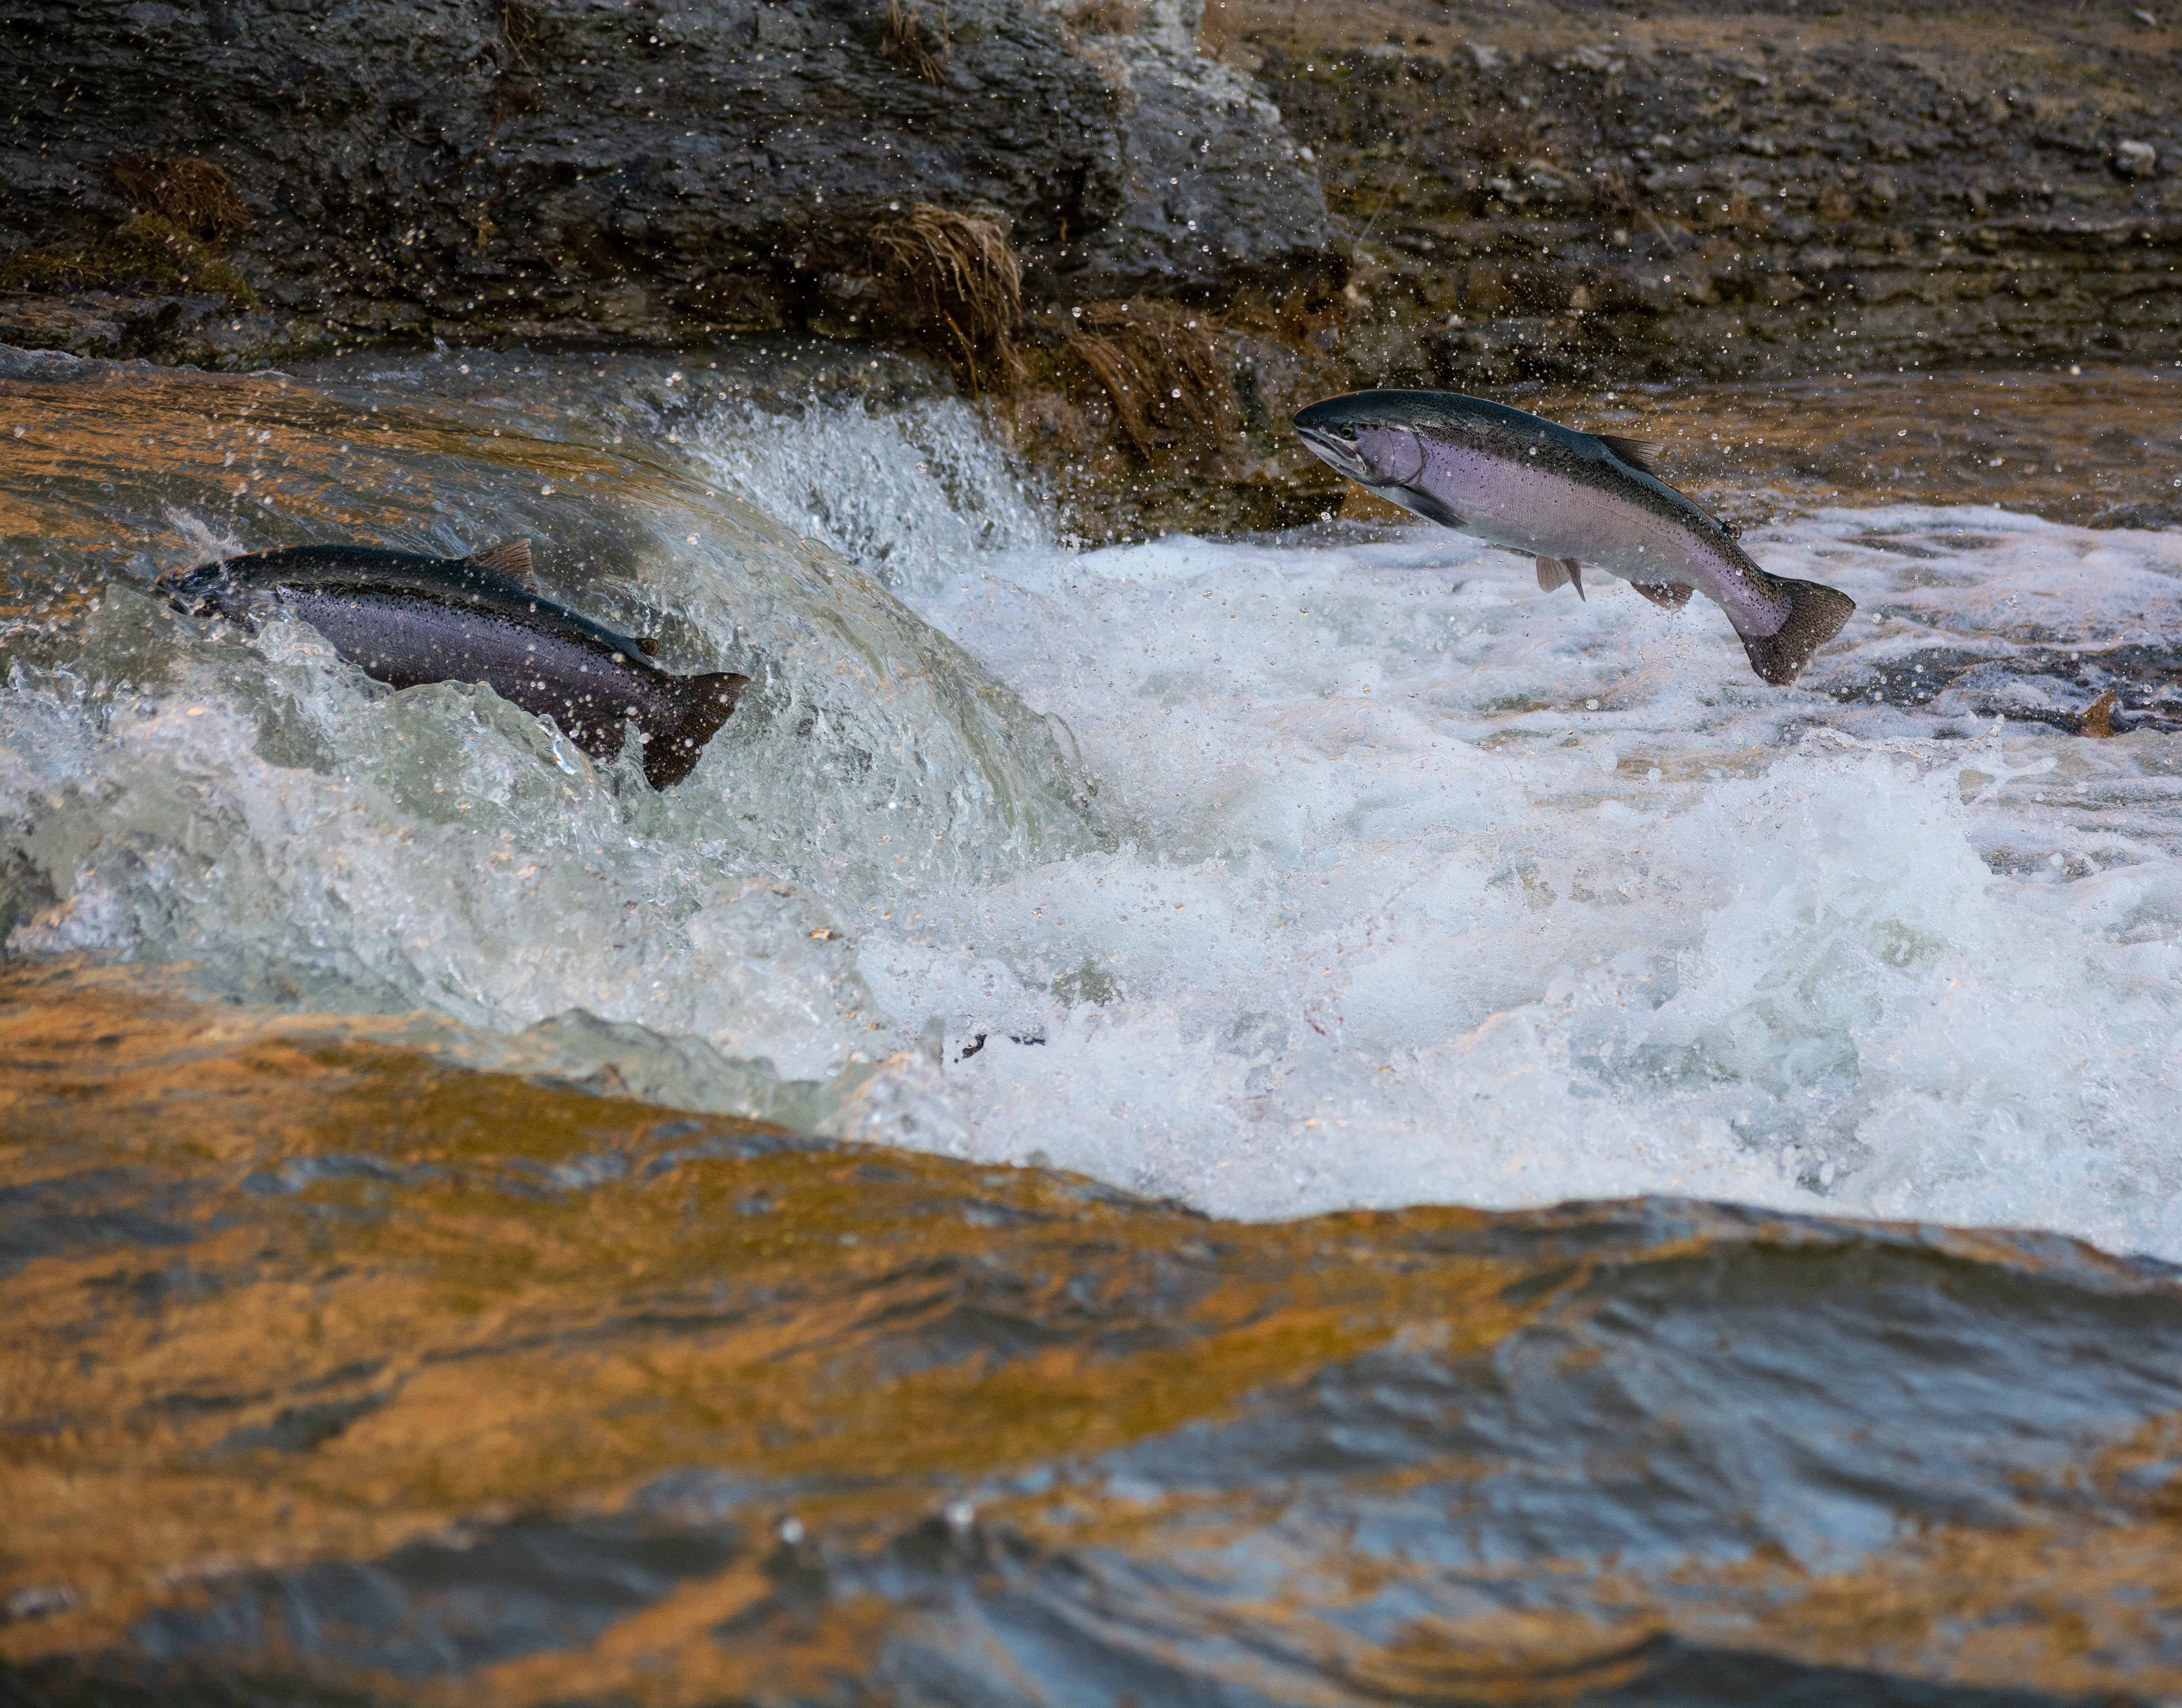
\includegraphics{spawn.jpg}

\bookmarksetup{startatroot}

\chapter*{Project Overview}\label{project-overview}
\addcontentsline{toc}{chapter}{Project Overview}

\markboth{Project Overview}{Project Overview}

\section*{Plan Purpose, Approach, and
Scope}\label{plan-purpose-approach-and-scope}
\addcontentsline{toc}{section}{Plan Purpose, Approach, and Scope}

\markright{Plan Purpose, Approach, and Scope}

The following Reconnecting our Rivers project represents the culmination
of a collaborative planning effort with the Confederacy of Mainland
Mi'kmaq (CMM) and the Canadian Wildlife Federation (CWF). The overall
aim is to build meaningful partnerships, reduce the threat of aquatic
barriers to diadromous fish and the livelihoods that they support. This
plan will identify priority actions that CMM, CWF, and other project
partners propose to undertake between 2023-2033 to preserve and restore
fish connectively in the Maqmekwitk (St.~Croix) watershed, with
additional watersheds being added in future years (including
Shubenacadie and Stewiacke River). This will be done through addressing
physical barriers to fish passage. This watershed connectivity plan will
be shared with local First Nations, Fisheries and Oceans Canada (DFO),
the NS Government, NGOs, and local stakeholders to inform directed
efforts to improve fish productivity and diversity in these
watersheds.\,

\section*{Vision Statement}\label{vision-statement}
\addcontentsline{toc}{section}{Vision Statement}

\markright{Vision Statement}

Healthy, well-connected rivers within the Maqmekwitk watershed support
populations of migratory fish including Plamu (Atlantic Salmon) and
Kataq (American Eel), improving the overall ecosystem health of the
watershed. In turn, these fish provide the continued food, social, and
ceremonial (FSC) needs of the Mi'kmaw people, as they have since time
immemorial. Both residents and visitors to the watershed will work
together, guided by the principles of Etuaptmumk (two-eyed seeing), to
mitigate the negative effects of anthropogenic aquatic barriers,
improving the resiliency of the watershed for the benefit and
appreciation of all.

\section*{Project Scope}\label{project-scope}
\addcontentsline{toc}{section}{Project Scope}

\markright{Project Scope}

Connectivity is a critical component of freshwater ecosystems that
encompasses a variety of factors related to ecosystem structure and
function, such as the ability of aquatic organisms to disperse and/or
migrate, the transportation of energy and matter (e.g., nutrient cycling
and sediment flows), and temperature regulation (Seliger and Zeiringer
(2018)). Though each of these factors are important when considering the
health of a watershed, for the purpose of this project the term
``connectivity'' is defined as the degree to which aquatic organisms can
disperse and/or migrate freely through freshwater systems. Within this
context, connectivity is primarily constrained by physical barriers,
including anthropogenic infrastructure such as dams and stream
crossings, and natural features such as waterfalls. This plan will focus
on the direct rehabilitation and prevention of localized, physical
barriers instead of the broad, land-use patterns causing chronic
connectivity issues in the watershed. The planning team decided that the
primary focus of this watershed connectivity plan is addressing barriers
to longitudinal connectivity (i.e., along the upstream-downstream plane)
due to the importance of maintaining fish passage to spawning and
rearing habitat in the watershed.

\section*{Focal species}\label{focal-species}
\addcontentsline{toc}{section}{Focal species}

\markright{Focal species}

Focal species represent the ecologically and culturally important
species for which habitat connectivity is being directly conserved
and/or restored in the watershed. The planning team selected three
target species: Plamu (Atlantic Salmon) and Kataq (American Eel). The
selection of these key species was driven primarily by local
conservation goals.

\subsection*{\texorpdfstring{Atlantic Salmon \textbar{} Plamu \textbar{}
\emph{Salmo
salar}}{Atlantic Salmon \textbar{} Plamu \textbar{} Salmo salar}}\label{atlantic-salmon-plamu-salmo-salar}
\addcontentsline{toc}{subsection}{Atlantic Salmon \textbar{} Plamu
\textbar{} \emph{Salmo salar}}

Atlantic Salmon are anadromous fishes, meaning mature adults spawn in
freshwater and juveniles rear in freshwater before undergoing a process
called smoltification where they migrate out to the ocean for 1-3+ years
before returning to the freshwater to repeat this process. Due to this
migratory process, salmon require unimpeded access between the ocean and
freshwater habitats to complete their life cycle.

Atlantic Salmon spawn in the pool-riffle transition zones of the main
stem and larger tributaries of a river (B, Bonzom, and E (2000);
Finstad, Armstrong, and Nislow (2010)). Within these stretches, they
seek out the tails of pools, where substrate size allows for females to
excavate a space to deposit the eggs to incubate below gravel beds. Fast
flowing, well oxygenated water with minimal fine sediments helps to
maximize successful embryo development. Atlantic Salmon juveniles (fry
and parr) rear in habitat that is deeper and slower, to facilitate their
weaker swimming and predation capabilities. Water depth, velocity, and
substrate size tend to increase with parr as they increase in size and
age. Shelter, in the form of large rocks, boulders, or overhead cover
provide crucial refuge for overwintering habitat. Channel gradients most
typically associated with these preferred spawning and rearing habitats
range from 0.12 to 25\%; with highest concentrations below 3\% (Amiro
(1993)).

Salmon in the St.~Croix watershed are a part of the Inner Bay of Fundy
population that was last assessed by Committee on the Status of
Endangered Wildlife in Canada (COSEWIC) as Endangered in 2010 (COSEWIC
(2010)) and has been listed on the Schedule 1 of the Species at Risk Act
since 2003.

\subsection*{\texorpdfstring{American Eel \textbar{} Kataq \textbar{}
\emph{Anguilla
rostrata}}{American Eel \textbar{} Kataq \textbar{} Anguilla rostrata}}\label{american-eel-kataq-anguilla-rostrata}
\addcontentsline{toc}{subsection}{American Eel \textbar{} Kataq
\textbar{} \emph{Anguilla rostrata}}

American Eel are catadromous species, meaning they spawn in the Sargasso
Sea and drift with the ocean currents towards the continental shelf as
glass eels. Elvers then continue migrating towards freshwater
tributaries to feed and mature, although some populations have been
known to stay in the estuaries and bays or move between freshwater and
estuary habitat over their life cycle. Their ability to tolerate a wide
variety of salinities and temperature thresholds allows them to occupy a
variety of habitat types.

American Eel are widely distributed throughout Nova Scotia rivers,
including the St.~Croix, and occupy freshwater habitat and estuary
habitat for feeding (on small fish, mollusks, insects, and crustaceans)
and growth. American Eel were assessed as Threatened by COSEWIC in 2012
(COSEWIC (2012)).

\section*{Geographic Scope}\label{geographic-scope}
\addcontentsline{toc}{section}{Geographic Scope}

\markright{Geographic Scope}

The primary geographic scope of this watershed connectivity plan is the
Maqmekwitk (St.~Croix), which is the larger branch of the Amaqapskiket
(Avon River) and drains into the Minas Basin, Bay of Fundy, NS. There
are three main branches of the Maqmekwitk, the branch that passes
through Panuk, the Herbert River, and the Miluamkitk (Meander River).
The Maqmekwitk has a total drainage area of 746.7 km2
(Figure~\ref{fig-geoscope}).

\begin{figure}

\centering{

\includegraphics{content/images/geo-scope-cmm.png}

}

\caption{\label{fig-geoscope}The primary geographic scope, the
Maqmekwitk (St.~Croix) watershed.}

\end{figure}%

The geographic scope of this project was further refined by identifying
naturally accessible waterbodies, which are defined as streams, lakes,
or reservoirs that target species would access in the absence of
anthropogenic barriers (Figure~\ref{fig-2}). Naturally accessible
waterbodies were spatially delineated using stream characteristics that
define the upper limit of their movement based on species-specific
swimming abilities (Table~\ref{tbl-spn}). While waterfalls
\textgreater5m were used as the upper limit for Atlantic Salmon
accessibility, our ability to comprehensively model this was limited by
incomplete height data for all waterfalls. Future iterations of this
project will include field assessment and compilation of local knowledge
of waterfall height to further define these boundaries. The spatial
extent of the naturally accessible waterbodies layer was then refined
based on existing fish observation data and/or redd surveys (for
Atlantic Salmon). These maps were explored by the planning team to
incorporate additional local knowledge, ensure accuracy, and finalize
the criteria used to define naturally accessible waterbodies. The new
geographic scope formed the foundation for all subsequent analyses and
planning steps.

\begin{longtable}[]{@{}lll@{}}

\caption{\label{tbl-spn}Species-specific stream characteristics used to
spatially delineate naturally accessible waterbodies and key habitat for
Atlantic Salmon and American Eel.}

\tabularnewline

\caption{}\label{T_03c92}\tabularnewline
\toprule\noalign{}
Species & Accessibility Parameters & Key Habitat Parameters \\
\midrule\noalign{}
\endfirsthead
\toprule\noalign{}
Species & Accessibility Parameters & Key Habitat Parameters \\
\midrule\noalign{}
\endhead
\bottomrule\noalign{}
\endlastfoot
Plamu, Atlantic Salmon~ & Channel gradient \textless30\%; waterfalls
\textless5m~ & Channel gradient \textless3\%~ \\
Kataq, American Eel~ & All stream segments~ & Strahler order 2+~ \\

\end{longtable}

\begin{figure}

\centering{

\includegraphics{content/images/figure_2.png}

}

\caption{\label{fig-2}Key habitat (channel gradient \textless3\%) and
naturally accessible waterbodies (\textless30\% channel gradient and
\textless5m waterfalls) to Plamu (Atlantic Salmon) within the Maqmekwitk
(St.~Croix) watershed.}

\end{figure}%

\begin{figure}

\centering{

\includegraphics{content/images/figure_3.png}

}

\caption{\label{fig-3}Key habitat (strahler order 2+) and naturally
accessible waterbodies (all stream segments) to Kataq (American Eel)
within the Maqmekwitk (St.~Croix) watershed.}

\end{figure}%

\section*{Structure Types}\label{structure-types}
\addcontentsline{toc}{section}{Structure Types}

\markright{Structure Types}

The following section highlights three main anthropogenic structure
types (aboiteaux, dams, and stream crossings) that fragment key habitat
for Plamu and Kataq in the Maqmekwitk watershed. .

\subsection*{Aboiteaux}\label{aboiteaux}
\addcontentsline{toc}{subsection}{Aboiteaux}

There are three modelled aboiteaux in the Maqmekwitk, each located close
to the mouth of the Minas Basin. There may be more aboiteaux identified
currently as stream crossings, but these will require further knowledge
exchange, data review and field assessments to confirm. One aboiteau is
a confirmed barrier but is low priority due to the low-quality upstream
habitat and difficulty in addressing this barrier type.

\subsection*{Dams}\label{dams}
\addcontentsline{toc}{subsection}{Dams}

There are seven mapped dams that potentially block a combined 154 km of
linear salmon and eel habitat in the Maqmekwitk. One smaller dam is
located downstream of Fundy Gypsum Mine Yard, one is unknown and
requires a field assessment, and five generate hydroelectricity. A set
of three hydroelectric dams owned and operated by Minas Energy block the
largest proportion of salmon habitat (39\%; \textasciitilde119km of
linear habitat) amongst all modelled structure types in the Maqmekwitk
watershed.

\subsection*{Stream Crossings}\label{stream-crossings}
\addcontentsline{toc}{subsection}{Stream Crossings}

Stream crossings (i.e., culverts) are the most abundant barrier type in
the watershed, with 485 stream crossings located downstream of modelled
key habitat for Plamu or Kataq. Stream crossings fully or partially
block 385 km of salmon and eel habitat. Detailed assessments by CMM were
previously completed on 82 stream crossings located downstream of salmon
and eel key habitat. Of these 82 structures, nine were in the top 30
ranked sets.

\bookmarksetup{startatroot}

\chapter*{Connectivity Status
Assessment}\label{connectivity-status-assessment}
\addcontentsline{toc}{chapter}{Connectivity Status Assessment}

\markboth{Connectivity Status Assessment}{Connectivity Status
Assessment}

\section*{Connectivity Status
Assessment}\label{connectivity-status-assessment-1}
\addcontentsline{toc}{section}{Connectivity Status Assessment}

\markright{Connectivity Status Assessment}

The current connectivity status for each species was estimated using
three spatial models:

\begin{enumerate}
\def\labelenumi{\arabic{enumi}.}
\item
  \textbf{Accessibility model:} Naturally accessible waterbodies are
  those that are considered likely accessible to focal species if no
  human-made barriers existed on the landscape. These were spatially
  delineated for each focal species using natural barriers (i.e.,
  waterfalls, gradient barriers, or subsurface flows) that would limit
  upstream movement (Table~\ref{tbl-spn}).
\item
  \textbf{Habitat model:} A subset of the naturally accessible waterbody
  layer was defined as key habitat based on the KEA. The habitat model
  identifies waterbodies that have a higher potential to support key
  habitat based on stream characteristics like channel gradient and
  discharge. The habitat model criteria can be found in
  (Table~\ref{tbl-spn}).
\item
  \textbf{Connectivity model:} A layer of known or modelled structures
  was overlaid on the key habitat results. Structures with unknown
  passability were treated as a full barrier until confirmed passable
  (100\% passable) or partially passable (25, 50, or 75\%) by either
  local knowledge, desktop review, or field assessment. Watershed
  connectivity was estimated by calculating the amount of key habitat
  that is connected to the ocean (i.e., not fragmented by human-made
  barriers). Key habitat with only passable structures downstream was
  considered fully connected. All key habitat with any full barrier
  downstream was considered disconnected.
\end{enumerate}

All connected habitats were summed and divided by the total amount of
key habitat in the watershed to determine the proportion of connected
habitat relative to the entire watershed. Of the estimated 758 km of key
spawning and rearing habitat for Plamu in the Maqmekwitk watershed,
30.54\% (231.6 km) is connected to the ocean (Figure~\ref{fig-4}).
Similarly, of the 464.9 km of key eel habitat (used for feeding and
growth) in the Maqmekwitk watershed, 32.71\% (152 km) is connected to
the ocean (Figure~\ref{fig-5}). These values are likely an underestimate
of how connected the system, and additional field assessments and local
knowledge exchange to confirm species-specific passability for potential
barriers will help to close those knowledge gaps and ensure a more
accurate estimate of connectivity status.

\begin{figure}

\centering{

\includegraphics{content/images/figure_4.png}

}

\caption{\label{fig-4}Connected (light blue) and disconnected (red) key
habitat for Plamu in the Maqmekwitk watershed. Atlantic Salmon
connectivity status was estimated as 30.54\%.}

\end{figure}%

\begin{figure}

\centering{

\includegraphics{content/images/figure_5.png}

}

\caption{\label{fig-5}Connected (light blue) and disconnected (red) key
habitat for Kataq in the Maqmekwitk watershed. American Eel connectivity
status was estimated as 32.71\%.}

\end{figure}%

\bookmarksetup{startatroot}

\chapter*{Barrier Prioritization}\label{barrier-prioritization}
\addcontentsline{toc}{chapter}{Barrier Prioritization}

\markboth{Barrier Prioritization}{Barrier Prioritization}

\section*{Maqmekwitk (St.~Croix) Watershed Barrier Prioritization
Summary}\label{maqmekwitk-st.-croix-watershed-barrier-prioritization-summary}
\addcontentsline{toc}{section}{Maqmekwitk (St.~Croix) Watershed Barrier
Prioritization Summary}

\markright{Maqmekwitk (St.~Croix) Watershed Barrier Prioritization
Summary}

The primary goal of Reconnecting our Rivers is to restore connectivity
to Plamu and Kataq habitat in the Maqmekwitk watershed. To achieve this
goal, the plan will guide which structures to assess in the field, and
subsequently, which barriers to address (i.e., remove or replace the
barrier, or temporarily add fish passage). To maximize conservation
efforts/resources towards achieving this goal, it is imperative to
identify a suite of barriers that, if addressed, will provide the
largest, most important contribution towards restored connectivity of
salmon and eel habitat. The following section outlines the ranking
process to identify the list of barriers.

\section*{Field Assessment Ranking
Process}\label{field-assessment-ranking-process}
\addcontentsline{toc}{section}{Field Assessment Ranking Process}

\markright{Field Assessment Ranking Process}

After all existing data and knowledge are collated for known and
modelled crossings, an iterative ranking process was conducted. The
ranking process is primarily used to guide field assessments and
maximize efficiency in ground truthing data/knowledge inputs and model
outputs, while providing a secondary purpose to evaluate the relative
key habitat gains of confirmed barriers in the watershed. Field
assessments can include an assessment of either the passability status
of a structure (whether fish can pass upstream, and to what degree),
whether the upstream habitat is suitable for the focal species, and
whether there are other undocumented anthropogenic or natural barriers
upstream or downstream. First, structures are grouped into `sets'. Sets
are identified by maximizing the key habitat gain for barriers in the
same tributary system. If adding a structure to a set reduces the
gain-per-barrier (i.e., the total habitat gain of the set divided by the
number of barriers in the set), then it is excluded and will be
considered part of another set. This results in sets ranging from one to
five structures (see Appendix A for more details on this process). Then,
each set is ranked by its potential to contribute to restoring the
overall habitat connectivity. The higher a set is ranked, the more
potential contribution it makes to restoring the overall habitat
connectivity, therefore making the set a higher priority for field
assessment. By assessing the passability status and upstream habitat of
the top-ranked sets, we close knowledge gaps with the greatest influence
on the overall connectivity model results.

Sets are ranked by a combination of two factors:

\begin{enumerate}
\def\labelenumi{\arabic{enumi}.}
\item
  The \textbf{long-term potential} impact that restoring connectivity at
  that structure could have on the overall connectivity status. This was
  measured by calculating and ranking sets by the amount of total
  upstream key habitat (i.e., ignoring any additional upstream sets).
  This ranking identifies sets that would have the greatest long-term
  potential gain in habitat connectivity once any subsequent upstream
  barriers are addressed.
\item
  The \textbf{immediate potential} impact that restoring connectivity at
  that structure could have on the overall connectivity status. This was
  measured by calculating the amount of functional upstream habitat
  (i.e., key habitat between that set and the next upstream set of
  structures). Sets were then ranked by functional upstream habitat
  amount in tiers, where sets with no downstream sets were ranked first,
  then sets with one downstream set, and so on. This ranking identifies
  sets that have the greatest immediate potential gain in habitat by
  prioritizing sets that do not rely on rehabilitation of downstream or
  upstream sets to realize these gains.
\end{enumerate}

An overall ranking for each set was produced as a composite of the
long-term and immediate potential gain ranks to prioritize sets that
maximize long-term and immediate potential to improve key habitat
connectivity in the watershed. All structures in the watershed
(excluding those confirmed as passable) were ranked and a subset of
those structures were selected by the planning team to assess in the
2023 field season.

\section*{Summary}\label{summary}
\addcontentsline{toc}{section}{Summary}

\markright{Summary}

Following field assessments, structures are placed on one of five
possible lists:

\begin{enumerate}
\def\labelenumi{\arabic{enumi}.}
\item
  \textbf{Priority barriers list} -- the structure is confirmed as 0,
  25, 50, or 75\% passable, has key habitat confirmed to exist upstream,
  and is considered actionable by the planning team (i.e., action items
  will be identified to address passability of the barrier). Depending
  on the barrier, owner, financial constraints, and quality of upstream
  habitat, the action may be to leave to end of life cycle before
  reviewing again, remove and decommission the road, replace with a new
  passable structure, or modify to temporarily restore connectivity
  (e.g., fish ladder or baffles installed (\{numref\}Table2).
\item
  \textbf{Assessed structures that remain data deficient list} -- some
  form of field assessment has been completed on the structure, but
  further investigation is required to confirm either the passability
  status or upstream habitat (\{numref\}Table3).
\item
  \textbf{Rehabilitated barriers list} -- priority barriers that have
  been addressed (either through removal, replacement, or temporary fish
  passage improvement projects (\{numref\}Table 4).
\item
  \textbf{Non-actionable barriers list} -- the structure is confirmed to
  be a barrier to fish passage and have some amount/quality of habitat
  upstream, but the planning team will not identify actions to address
  passability of the barrier because of logistic considerations (e.g.,
  financial costs), short habitat gain, or the upstream habitat is of
  poor quality or unsuitable in its present condition to support key
  life stages of the focal species (Appendix B).
\item
  \textbf{Excluded structures list} -- the structure is excluded from
  further consideration in subsequent ranking and work planning because
  the structure is confirmed passable (e.g., bridge), not present, or
  there is no key habitat upstream (Appendix B).
\end{enumerate}

\global\setlength{\Oldarrayrulewidth}{\arrayrulewidth}

\global\setlength{\Oldtabcolsep}{\tabcolsep}

\setlength{\tabcolsep}{0pt}

\renewcommand*{\arraystretch}{1.5}



\providecommand{\ascline}[3]{\noalign{\global\arrayrulewidth #1}\arrayrulecolor[HTML]{#2}\cline{#3}}

\begin{longtable}[c]{|p{3.20in}|p{4.08in}|p{1.60in}|p{1.89in}|p{1.84in}|p{1.84in}|p{1.84in}|p{0.74in}|p{1.87in}|p{2.33in}|p{3.19in}|p{2.33in}|p{3.19in}|p{1.99in}|p{0.83in}|p{2.08in}|p{13.27in}|p{17.01in}}

\caption{\label{tbl-priority}The Maqmekwitk watershed priority barrier
list, which includes barriers that have undergone field assessment, been
reviewed by the planning team, and selected to be addressed (whether
removed, replaced with a passable structure, or provided temporary fish
passage).}

\tabularnewline

\hhline{>{\arrayrulecolor[HTML]{666666}\global\arrayrulewidth=1.5pt}->{\arrayrulecolor[HTML]{666666}\global\arrayrulewidth=1.5pt}->{\arrayrulecolor[HTML]{666666}\global\arrayrulewidth=1.5pt}->{\arrayrulecolor[HTML]{666666}\global\arrayrulewidth=1.5pt}->{\arrayrulecolor[HTML]{666666}\global\arrayrulewidth=1.5pt}->{\arrayrulecolor[HTML]{666666}\global\arrayrulewidth=1.5pt}->{\arrayrulecolor[HTML]{666666}\global\arrayrulewidth=1.5pt}->{\arrayrulecolor[HTML]{666666}\global\arrayrulewidth=1.5pt}->{\arrayrulecolor[HTML]{666666}\global\arrayrulewidth=1.5pt}->{\arrayrulecolor[HTML]{666666}\global\arrayrulewidth=1.5pt}->{\arrayrulecolor[HTML]{666666}\global\arrayrulewidth=1.5pt}->{\arrayrulecolor[HTML]{666666}\global\arrayrulewidth=1.5pt}->{\arrayrulecolor[HTML]{666666}\global\arrayrulewidth=1.5pt}->{\arrayrulecolor[HTML]{666666}\global\arrayrulewidth=1.5pt}->{\arrayrulecolor[HTML]{666666}\global\arrayrulewidth=1.5pt}->{\arrayrulecolor[HTML]{666666}\global\arrayrulewidth=1.5pt}->{\arrayrulecolor[HTML]{666666}\global\arrayrulewidth=1.5pt}->{\arrayrulecolor[HTML]{666666}\global\arrayrulewidth=1.5pt}-}

\multicolumn{1}{>{\cellcolor[HTML]{008270}\raggedright}m{\dimexpr 3.2in+0\tabcolsep}}{\textcolor[HTML]{FFFFFF}{\fontsize{11}{11}\selectfont{Barrier\ ID}}} & \multicolumn{1}{>{\cellcolor[HTML]{008270}\raggedright}m{\dimexpr 4.08in+0\tabcolsep}}{\textcolor[HTML]{FFFFFF}{\fontsize{11}{11}\selectfont{Internal\ Name}}} & \multicolumn{1}{>{\cellcolor[HTML]{008270}\raggedright}m{\dimexpr 1.6in+0\tabcolsep}}{\textcolor[HTML]{FFFFFF}{\fontsize{11}{11}\selectfont{Watercourse\ Name}}} & \multicolumn{1}{>{\cellcolor[HTML]{008270}\raggedright}m{\dimexpr 1.89in+0\tabcolsep}}{\textcolor[HTML]{FFFFFF}{\fontsize{11}{11}\selectfont{Road\ Name}}} & \multicolumn{1}{>{\cellcolor[HTML]{008270}\raggedright}m{\dimexpr 1.84in+0\tabcolsep}}{\textcolor[HTML]{FFFFFF}{\fontsize{11}{11}\selectfont{Structure\ Type}}} & \multicolumn{1}{>{\cellcolor[HTML]{008270}\raggedright}m{\dimexpr 1.84in+0\tabcolsep}}{\textcolor[HTML]{FFFFFF}{\fontsize{11}{11}\selectfont{Passability\ Status\ (AS)}}} & \multicolumn{1}{>{\cellcolor[HTML]{008270}\raggedright}m{\dimexpr 1.84in+0\tabcolsep}}{\textcolor[HTML]{FFFFFF}{\fontsize{11}{11}\selectfont{Passability\ Status\ (AE)}}} & \multicolumn{1}{>{\cellcolor[HTML]{008270}\raggedright}m{\dimexpr 0.74in+0\tabcolsep}}{\textcolor[HTML]{FFFFFF}{\fontsize{11}{11}\selectfont{Owner}}} & \multicolumn{1}{>{\cellcolor[HTML]{008270}\raggedright}m{\dimexpr 1.87in+0\tabcolsep}}{\textcolor[HTML]{FFFFFF}{\fontsize{11}{11}\selectfont{Number\ Barriers\ Group}}} & \multicolumn{1}{>{\cellcolor[HTML]{008270}\raggedright}m{\dimexpr 2.33in+0\tabcolsep}}{\textcolor[HTML]{FFFFFF}{\fontsize{11}{11}\selectfont{Total\ Habitat\ Gain\ Group\ (AS)}}} & \multicolumn{1}{>{\cellcolor[HTML]{008270}\raggedright}m{\dimexpr 3.19in+0\tabcolsep}}{\textcolor[HTML]{FFFFFF}{\fontsize{11}{11}\selectfont{Weighted\ Total\ Habitat\ Gained\ Group\ (AS)}}} & \multicolumn{1}{>{\cellcolor[HTML]{008270}\raggedright}m{\dimexpr 2.33in+0\tabcolsep}}{\textcolor[HTML]{FFFFFF}{\fontsize{11}{11}\selectfont{Total\ Habitat\ Gain\ Group\ (AE)}}} & \multicolumn{1}{>{\cellcolor[HTML]{008270}\raggedright}m{\dimexpr 3.19in+0\tabcolsep}}{\textcolor[HTML]{FFFFFF}{\fontsize{11}{11}\selectfont{Weighted\ Total\ Habitat\ Gained\ Group\ (AE)}}} & \multicolumn{1}{>{\cellcolor[HTML]{008270}\raggedright}m{\dimexpr 1.99in+0\tabcolsep}}{\textcolor[HTML]{FFFFFF}{\fontsize{11}{11}\selectfont{Upstream\ Habitat\ Quality}}} & \multicolumn{1}{>{\cellcolor[HTML]{008270}\raggedright}m{\dimexpr 0.83in+0\tabcolsep}}{\textcolor[HTML]{FFFFFF}{\fontsize{11}{11}\selectfont{Priority}}} & \multicolumn{1}{>{\cellcolor[HTML]{008270}\raggedright}m{\dimexpr 2.08in+0\tabcolsep}}{\textcolor[HTML]{FFFFFF}{\fontsize{11}{11}\selectfont{Next\ Steps}}} & \multicolumn{1}{>{\cellcolor[HTML]{008270}\raggedright}m{\dimexpr 13.27in+0\tabcolsep}}{\textcolor[HTML]{FFFFFF}{\fontsize{11}{11}\selectfont{Reason}}} & \multicolumn{1}{>{\cellcolor[HTML]{008270}\raggedright}m{\dimexpr 17.01in+0\tabcolsep}}{\textcolor[HTML]{FFFFFF}{\fontsize{11}{11}\selectfont{Notes}}} \\

\noalign{\global\arrayrulewidth 0pt}\arrayrulecolor[HTML]{000000}

\hhline{>{\arrayrulecolor[HTML]{666666}\global\arrayrulewidth=1.5pt}->{\arrayrulecolor[HTML]{666666}\global\arrayrulewidth=1.5pt}->{\arrayrulecolor[HTML]{666666}\global\arrayrulewidth=1.5pt}->{\arrayrulecolor[HTML]{666666}\global\arrayrulewidth=1.5pt}->{\arrayrulecolor[HTML]{666666}\global\arrayrulewidth=1.5pt}->{\arrayrulecolor[HTML]{666666}\global\arrayrulewidth=1.5pt}->{\arrayrulecolor[HTML]{666666}\global\arrayrulewidth=1.5pt}->{\arrayrulecolor[HTML]{666666}\global\arrayrulewidth=1.5pt}->{\arrayrulecolor[HTML]{666666}\global\arrayrulewidth=1.5pt}->{\arrayrulecolor[HTML]{666666}\global\arrayrulewidth=1.5pt}->{\arrayrulecolor[HTML]{666666}\global\arrayrulewidth=1.5pt}->{\arrayrulecolor[HTML]{666666}\global\arrayrulewidth=1.5pt}->{\arrayrulecolor[HTML]{666666}\global\arrayrulewidth=1.5pt}->{\arrayrulecolor[HTML]{666666}\global\arrayrulewidth=1.5pt}->{\arrayrulecolor[HTML]{666666}\global\arrayrulewidth=1.5pt}->{\arrayrulecolor[HTML]{666666}\global\arrayrulewidth=1.5pt}->{\arrayrulecolor[HTML]{666666}\global\arrayrulewidth=1.5pt}->{\arrayrulecolor[HTML]{666666}\global\arrayrulewidth=1.5pt}-}\endfirsthead 

\hhline{>{\arrayrulecolor[HTML]{666666}\global\arrayrulewidth=1.5pt}->{\arrayrulecolor[HTML]{666666}\global\arrayrulewidth=1.5pt}->{\arrayrulecolor[HTML]{666666}\global\arrayrulewidth=1.5pt}->{\arrayrulecolor[HTML]{666666}\global\arrayrulewidth=1.5pt}->{\arrayrulecolor[HTML]{666666}\global\arrayrulewidth=1.5pt}->{\arrayrulecolor[HTML]{666666}\global\arrayrulewidth=1.5pt}->{\arrayrulecolor[HTML]{666666}\global\arrayrulewidth=1.5pt}->{\arrayrulecolor[HTML]{666666}\global\arrayrulewidth=1.5pt}->{\arrayrulecolor[HTML]{666666}\global\arrayrulewidth=1.5pt}->{\arrayrulecolor[HTML]{666666}\global\arrayrulewidth=1.5pt}->{\arrayrulecolor[HTML]{666666}\global\arrayrulewidth=1.5pt}->{\arrayrulecolor[HTML]{666666}\global\arrayrulewidth=1.5pt}->{\arrayrulecolor[HTML]{666666}\global\arrayrulewidth=1.5pt}->{\arrayrulecolor[HTML]{666666}\global\arrayrulewidth=1.5pt}->{\arrayrulecolor[HTML]{666666}\global\arrayrulewidth=1.5pt}->{\arrayrulecolor[HTML]{666666}\global\arrayrulewidth=1.5pt}->{\arrayrulecolor[HTML]{666666}\global\arrayrulewidth=1.5pt}->{\arrayrulecolor[HTML]{666666}\global\arrayrulewidth=1.5pt}-}

\multicolumn{1}{>{\cellcolor[HTML]{008270}\raggedright}m{\dimexpr 3.2in+0\tabcolsep}}{\textcolor[HTML]{FFFFFF}{\fontsize{11}{11}\selectfont{Barrier\ ID}}} & \multicolumn{1}{>{\cellcolor[HTML]{008270}\raggedright}m{\dimexpr 4.08in+0\tabcolsep}}{\textcolor[HTML]{FFFFFF}{\fontsize{11}{11}\selectfont{Internal\ Name}}} & \multicolumn{1}{>{\cellcolor[HTML]{008270}\raggedright}m{\dimexpr 1.6in+0\tabcolsep}}{\textcolor[HTML]{FFFFFF}{\fontsize{11}{11}\selectfont{Watercourse\ Name}}} & \multicolumn{1}{>{\cellcolor[HTML]{008270}\raggedright}m{\dimexpr 1.89in+0\tabcolsep}}{\textcolor[HTML]{FFFFFF}{\fontsize{11}{11}\selectfont{Road\ Name}}} & \multicolumn{1}{>{\cellcolor[HTML]{008270}\raggedright}m{\dimexpr 1.84in+0\tabcolsep}}{\textcolor[HTML]{FFFFFF}{\fontsize{11}{11}\selectfont{Structure\ Type}}} & \multicolumn{1}{>{\cellcolor[HTML]{008270}\raggedright}m{\dimexpr 1.84in+0\tabcolsep}}{\textcolor[HTML]{FFFFFF}{\fontsize{11}{11}\selectfont{Passability\ Status\ (AS)}}} & \multicolumn{1}{>{\cellcolor[HTML]{008270}\raggedright}m{\dimexpr 1.84in+0\tabcolsep}}{\textcolor[HTML]{FFFFFF}{\fontsize{11}{11}\selectfont{Passability\ Status\ (AE)}}} & \multicolumn{1}{>{\cellcolor[HTML]{008270}\raggedright}m{\dimexpr 0.74in+0\tabcolsep}}{\textcolor[HTML]{FFFFFF}{\fontsize{11}{11}\selectfont{Owner}}} & \multicolumn{1}{>{\cellcolor[HTML]{008270}\raggedright}m{\dimexpr 1.87in+0\tabcolsep}}{\textcolor[HTML]{FFFFFF}{\fontsize{11}{11}\selectfont{Number\ Barriers\ Group}}} & \multicolumn{1}{>{\cellcolor[HTML]{008270}\raggedright}m{\dimexpr 2.33in+0\tabcolsep}}{\textcolor[HTML]{FFFFFF}{\fontsize{11}{11}\selectfont{Total\ Habitat\ Gain\ Group\ (AS)}}} & \multicolumn{1}{>{\cellcolor[HTML]{008270}\raggedright}m{\dimexpr 3.19in+0\tabcolsep}}{\textcolor[HTML]{FFFFFF}{\fontsize{11}{11}\selectfont{Weighted\ Total\ Habitat\ Gained\ Group\ (AS)}}} & \multicolumn{1}{>{\cellcolor[HTML]{008270}\raggedright}m{\dimexpr 2.33in+0\tabcolsep}}{\textcolor[HTML]{FFFFFF}{\fontsize{11}{11}\selectfont{Total\ Habitat\ Gain\ Group\ (AE)}}} & \multicolumn{1}{>{\cellcolor[HTML]{008270}\raggedright}m{\dimexpr 3.19in+0\tabcolsep}}{\textcolor[HTML]{FFFFFF}{\fontsize{11}{11}\selectfont{Weighted\ Total\ Habitat\ Gained\ Group\ (AE)}}} & \multicolumn{1}{>{\cellcolor[HTML]{008270}\raggedright}m{\dimexpr 1.99in+0\tabcolsep}}{\textcolor[HTML]{FFFFFF}{\fontsize{11}{11}\selectfont{Upstream\ Habitat\ Quality}}} & \multicolumn{1}{>{\cellcolor[HTML]{008270}\raggedright}m{\dimexpr 0.83in+0\tabcolsep}}{\textcolor[HTML]{FFFFFF}{\fontsize{11}{11}\selectfont{Priority}}} & \multicolumn{1}{>{\cellcolor[HTML]{008270}\raggedright}m{\dimexpr 2.08in+0\tabcolsep}}{\textcolor[HTML]{FFFFFF}{\fontsize{11}{11}\selectfont{Next\ Steps}}} & \multicolumn{1}{>{\cellcolor[HTML]{008270}\raggedright}m{\dimexpr 13.27in+0\tabcolsep}}{\textcolor[HTML]{FFFFFF}{\fontsize{11}{11}\selectfont{Reason}}} & \multicolumn{1}{>{\cellcolor[HTML]{008270}\raggedright}m{\dimexpr 17.01in+0\tabcolsep}}{\textcolor[HTML]{FFFFFF}{\fontsize{11}{11}\selectfont{Notes}}} \\

\noalign{\global\arrayrulewidth 0pt}\arrayrulecolor[HTML]{000000}

\hhline{>{\arrayrulecolor[HTML]{666666}\global\arrayrulewidth=1.5pt}->{\arrayrulecolor[HTML]{666666}\global\arrayrulewidth=1.5pt}->{\arrayrulecolor[HTML]{666666}\global\arrayrulewidth=1.5pt}->{\arrayrulecolor[HTML]{666666}\global\arrayrulewidth=1.5pt}->{\arrayrulecolor[HTML]{666666}\global\arrayrulewidth=1.5pt}->{\arrayrulecolor[HTML]{666666}\global\arrayrulewidth=1.5pt}->{\arrayrulecolor[HTML]{666666}\global\arrayrulewidth=1.5pt}->{\arrayrulecolor[HTML]{666666}\global\arrayrulewidth=1.5pt}->{\arrayrulecolor[HTML]{666666}\global\arrayrulewidth=1.5pt}->{\arrayrulecolor[HTML]{666666}\global\arrayrulewidth=1.5pt}->{\arrayrulecolor[HTML]{666666}\global\arrayrulewidth=1.5pt}->{\arrayrulecolor[HTML]{666666}\global\arrayrulewidth=1.5pt}->{\arrayrulecolor[HTML]{666666}\global\arrayrulewidth=1.5pt}->{\arrayrulecolor[HTML]{666666}\global\arrayrulewidth=1.5pt}->{\arrayrulecolor[HTML]{666666}\global\arrayrulewidth=1.5pt}->{\arrayrulecolor[HTML]{666666}\global\arrayrulewidth=1.5pt}->{\arrayrulecolor[HTML]{666666}\global\arrayrulewidth=1.5pt}->{\arrayrulecolor[HTML]{666666}\global\arrayrulewidth=1.5pt}-}\endhead



\multicolumn{1}{>{\raggedright}m{\dimexpr 3.2in+0\tabcolsep}}{\textcolor[HTML]{000000}{\fontsize{11}{11}\selectfont{7df79d64-77e8-42a6-af8c-f7ae4cbd5e9f}}} & \multicolumn{1}{>{\raggedright}m{\dimexpr 4.08in+0\tabcolsep}}{\textcolor[HTML]{000000}{\fontsize{11}{11}\selectfont{Lower\ St.\ Croix\ -\ hydroelectric\ facility}}} & \multicolumn{1}{>{\raggedright}m{\dimexpr 1.6in+0\tabcolsep}}{\textcolor[HTML]{000000}{\fontsize{11}{11}\selectfont{St.\ Croix}}} & \multicolumn{1}{>{\raggedright}m{\dimexpr 1.89in+0\tabcolsep}}{\textcolor[HTML]{000000}{\fontsize{11}{11}\selectfont{Evangaline\ Trail}}} & \multicolumn{1}{>{\raggedright}m{\dimexpr 1.84in+0\tabcolsep}}{\textcolor[HTML]{000000}{\fontsize{11}{11}\selectfont{Dam}}} & \multicolumn{1}{>{\raggedright}m{\dimexpr 1.84in+0\tabcolsep}}{\textcolor[HTML]{000000}{\fontsize{11}{11}\selectfont{0}}} & \multicolumn{1}{>{\raggedright}m{\dimexpr 1.84in+0\tabcolsep}}{\textcolor[HTML]{000000}{\fontsize{11}{11}\selectfont{0}}} & \multicolumn{1}{>{\raggedright}m{\dimexpr 0.74in+0\tabcolsep}}{\textcolor[HTML]{000000}{\fontsize{11}{11}\selectfont{}}} & \multicolumn{1}{>{\raggedright}m{\dimexpr 1.87in+0\tabcolsep}}{\textcolor[HTML]{000000}{\fontsize{11}{11}\selectfont{3}}} & \multicolumn{1}{>{\raggedright}m{\dimexpr 2.33in+0\tabcolsep}}{\textcolor[HTML]{000000}{\fontsize{11}{11}\selectfont{119.936801}}} & \multicolumn{1}{>{\raggedright}m{\dimexpr 3.19in+0\tabcolsep}}{\textcolor[HTML]{000000}{\fontsize{11}{11}\selectfont{91.734697}}} & \multicolumn{1}{>{\raggedright}m{\dimexpr 2.33in+0\tabcolsep}}{\textcolor[HTML]{000000}{\fontsize{11}{11}\selectfont{96.856772}}} & \multicolumn{1}{>{\raggedright}m{\dimexpr 3.19in+0\tabcolsep}}{\textcolor[HTML]{000000}{\fontsize{11}{11}\selectfont{90.738809}}} & \multicolumn{1}{>{\raggedright}m{\dimexpr 1.99in+0\tabcolsep}}{\textcolor[HTML]{000000}{\fontsize{11}{11}\selectfont{}}} & \multicolumn{1}{>{\raggedright}m{\dimexpr 0.83in+0\tabcolsep}}{\textcolor[HTML]{000000}{\fontsize{11}{11}\selectfont{High}}} & \multicolumn{1}{>{\raggedright}m{\dimexpr 2.08in+0\tabcolsep}}{\textcolor[HTML]{000000}{\fontsize{11}{11}\selectfont{Bring\ barrier\ to\ regulator}}} & \multicolumn{1}{>{\raggedright}m{\dimexpr 13.27in+0\tabcolsep}}{\textcolor[HTML]{000000}{\fontsize{11}{11}\selectfont{}}} & \multicolumn{1}{>{\raggedright}m{\dimexpr 17.01in+0\tabcolsep}}{\textcolor[HTML]{000000}{\fontsize{11}{11}\selectfont{need\ to\ submit\ a\ FOIPOP\ and\ ATIP}}} \\

\noalign{\global\arrayrulewidth 0pt}\arrayrulecolor[HTML]{000000}





\multicolumn{1}{>{\raggedright}m{\dimexpr 3.2in+0\tabcolsep}}{\textcolor[HTML]{000000}{\fontsize{11}{11}\selectfont{93c5a3a7-bb1c-462f-bf11-8b28f1083ea8}}} & \multicolumn{1}{>{\raggedright}m{\dimexpr 4.08in+0\tabcolsep}}{\textcolor[HTML]{000000}{\fontsize{11}{11}\selectfont{St.\ Croix\ hydroelectric\ facility}}} & \multicolumn{1}{>{\raggedright}m{\dimexpr 1.6in+0\tabcolsep}}{\textcolor[HTML]{000000}{\fontsize{11}{11}\selectfont{St.\ Croix}}} & \multicolumn{1}{>{\raggedright}m{\dimexpr 1.89in+0\tabcolsep}}{\textcolor[HTML]{000000}{\fontsize{11}{11}\selectfont{Salmon\ Hole\ Dam\ Rd}}} & \multicolumn{1}{>{\raggedright}m{\dimexpr 1.84in+0\tabcolsep}}{\textcolor[HTML]{000000}{\fontsize{11}{11}\selectfont{Dam}}} & \multicolumn{1}{>{\raggedright}m{\dimexpr 1.84in+0\tabcolsep}}{\textcolor[HTML]{000000}{\fontsize{11}{11}\selectfont{0}}} & \multicolumn{1}{>{\raggedright}m{\dimexpr 1.84in+0\tabcolsep}}{\textcolor[HTML]{000000}{\fontsize{11}{11}\selectfont{0}}} & \multicolumn{1}{>{\raggedright}m{\dimexpr 0.74in+0\tabcolsep}}{\textcolor[HTML]{000000}{\fontsize{11}{11}\selectfont{}}} & \multicolumn{1}{>{\raggedright}m{\dimexpr 1.87in+0\tabcolsep}}{\textcolor[HTML]{000000}{\fontsize{11}{11}\selectfont{3}}} & \multicolumn{1}{>{\raggedright}m{\dimexpr 2.33in+0\tabcolsep}}{\textcolor[HTML]{000000}{\fontsize{11}{11}\selectfont{119.936801}}} & \multicolumn{1}{>{\raggedright}m{\dimexpr 3.19in+0\tabcolsep}}{\textcolor[HTML]{000000}{\fontsize{11}{11}\selectfont{91.734697}}} & \multicolumn{1}{>{\raggedright}m{\dimexpr 2.33in+0\tabcolsep}}{\textcolor[HTML]{000000}{\fontsize{11}{11}\selectfont{96.856772}}} & \multicolumn{1}{>{\raggedright}m{\dimexpr 3.19in+0\tabcolsep}}{\textcolor[HTML]{000000}{\fontsize{11}{11}\selectfont{90.738809}}} & \multicolumn{1}{>{\raggedright}m{\dimexpr 1.99in+0\tabcolsep}}{\textcolor[HTML]{000000}{\fontsize{11}{11}\selectfont{}}} & \multicolumn{1}{>{\raggedright}m{\dimexpr 0.83in+0\tabcolsep}}{\textcolor[HTML]{000000}{\fontsize{11}{11}\selectfont{High}}} & \multicolumn{1}{>{\raggedright}m{\dimexpr 2.08in+0\tabcolsep}}{\textcolor[HTML]{000000}{\fontsize{11}{11}\selectfont{Bring\ barrier\ to\ regulator}}} & \multicolumn{1}{>{\raggedright}m{\dimexpr 13.27in+0\tabcolsep}}{\textcolor[HTML]{000000}{\fontsize{11}{11}\selectfont{}}} & \multicolumn{1}{>{\raggedright}m{\dimexpr 17.01in+0\tabcolsep}}{\textcolor[HTML]{000000}{\fontsize{11}{11}\selectfont{need\ to\ submit\ a\ FOIPOP\ and\ ATIP}}} \\

\noalign{\global\arrayrulewidth 0pt}\arrayrulecolor[HTML]{000000}





\multicolumn{1}{>{\raggedright}m{\dimexpr 3.2in+0\tabcolsep}}{\textcolor[HTML]{000000}{\fontsize{11}{11}\selectfont{4c4d6443-ba54-46dc-bf2c-51922ccb62cc}}} & \multicolumn{1}{>{\raggedright}m{\dimexpr 4.08in+0\tabcolsep}}{\textcolor[HTML]{000000}{\fontsize{11}{11}\selectfont{Upper\ St.\ Croix/Salmon\ Hole\ Dam\ -\ hydroelectric\ facility}}} & \multicolumn{1}{>{\raggedright}m{\dimexpr 1.6in+0\tabcolsep}}{\textcolor[HTML]{000000}{\fontsize{11}{11}\selectfont{St.\ Croix}}} & \multicolumn{1}{>{\raggedright}m{\dimexpr 1.89in+0\tabcolsep}}{\textcolor[HTML]{000000}{\fontsize{11}{11}\selectfont{Salmon\ Hole\ Dam\ Rd}}} & \multicolumn{1}{>{\raggedright}m{\dimexpr 1.84in+0\tabcolsep}}{\textcolor[HTML]{000000}{\fontsize{11}{11}\selectfont{Dam}}} & \multicolumn{1}{>{\raggedright}m{\dimexpr 1.84in+0\tabcolsep}}{\textcolor[HTML]{000000}{\fontsize{11}{11}\selectfont{0}}} & \multicolumn{1}{>{\raggedright}m{\dimexpr 1.84in+0\tabcolsep}}{\textcolor[HTML]{000000}{\fontsize{11}{11}\selectfont{0}}} & \multicolumn{1}{>{\raggedright}m{\dimexpr 0.74in+0\tabcolsep}}{\textcolor[HTML]{000000}{\fontsize{11}{11}\selectfont{}}} & \multicolumn{1}{>{\raggedright}m{\dimexpr 1.87in+0\tabcolsep}}{\textcolor[HTML]{000000}{\fontsize{11}{11}\selectfont{3}}} & \multicolumn{1}{>{\raggedright}m{\dimexpr 2.33in+0\tabcolsep}}{\textcolor[HTML]{000000}{\fontsize{11}{11}\selectfont{119.936801}}} & \multicolumn{1}{>{\raggedright}m{\dimexpr 3.19in+0\tabcolsep}}{\textcolor[HTML]{000000}{\fontsize{11}{11}\selectfont{91.734697}}} & \multicolumn{1}{>{\raggedright}m{\dimexpr 2.33in+0\tabcolsep}}{\textcolor[HTML]{000000}{\fontsize{11}{11}\selectfont{96.856772}}} & \multicolumn{1}{>{\raggedright}m{\dimexpr 3.19in+0\tabcolsep}}{\textcolor[HTML]{000000}{\fontsize{11}{11}\selectfont{90.738809}}} & \multicolumn{1}{>{\raggedright}m{\dimexpr 1.99in+0\tabcolsep}}{\textcolor[HTML]{000000}{\fontsize{11}{11}\selectfont{}}} & \multicolumn{1}{>{\raggedright}m{\dimexpr 0.83in+0\tabcolsep}}{\textcolor[HTML]{000000}{\fontsize{11}{11}\selectfont{High}}} & \multicolumn{1}{>{\raggedright}m{\dimexpr 2.08in+0\tabcolsep}}{\textcolor[HTML]{000000}{\fontsize{11}{11}\selectfont{Bring\ barrier\ to\ regulator}}} & \multicolumn{1}{>{\raggedright}m{\dimexpr 13.27in+0\tabcolsep}}{\textcolor[HTML]{000000}{\fontsize{11}{11}\selectfont{}}} & \multicolumn{1}{>{\raggedright}m{\dimexpr 17.01in+0\tabcolsep}}{\textcolor[HTML]{000000}{\fontsize{11}{11}\selectfont{need\ to\ submit\ a\ FOIPOP\ and\ ATIP}}} \\

\noalign{\global\arrayrulewidth 0pt}\arrayrulecolor[HTML]{000000}





\multicolumn{1}{>{\raggedright}m{\dimexpr 3.2in+0\tabcolsep}}{\textcolor[HTML]{000000}{\fontsize{11}{11}\selectfont{e4939efd-23a2-4fa7-9622-e5877d9b323c}}} & \multicolumn{1}{>{\raggedright}m{\dimexpr 4.08in+0\tabcolsep}}{\textcolor[HTML]{000000}{\fontsize{11}{11}\selectfont{}}} & \multicolumn{1}{>{\raggedright}m{\dimexpr 1.6in+0\tabcolsep}}{\textcolor[HTML]{000000}{\fontsize{11}{11}\selectfont{Shaw\ Brook}}} & \multicolumn{1}{>{\raggedright}m{\dimexpr 1.89in+0\tabcolsep}}{\textcolor[HTML]{000000}{\fontsize{11}{11}\selectfont{Avondale\ Road}}} & \multicolumn{1}{>{\raggedright}m{\dimexpr 1.84in+0\tabcolsep}}{\textcolor[HTML]{000000}{\fontsize{11}{11}\selectfont{Aboiteaux}}} & \multicolumn{1}{>{\raggedright}m{\dimexpr 1.84in+0\tabcolsep}}{\textcolor[HTML]{000000}{\fontsize{11}{11}\selectfont{0}}} & \multicolumn{1}{>{\raggedright}m{\dimexpr 1.84in+0\tabcolsep}}{\textcolor[HTML]{000000}{\fontsize{11}{11}\selectfont{0}}} & \multicolumn{1}{>{\raggedright}m{\dimexpr 0.74in+0\tabcolsep}}{\textcolor[HTML]{000000}{\fontsize{11}{11}\selectfont{}}} & \multicolumn{1}{>{\raggedright}m{\dimexpr 1.87in+0\tabcolsep}}{\textcolor[HTML]{000000}{\fontsize{11}{11}\selectfont{2}}} & \multicolumn{1}{>{\raggedright}m{\dimexpr 2.33in+0\tabcolsep}}{\textcolor[HTML]{000000}{\fontsize{11}{11}\selectfont{4.589670}}} & \multicolumn{1}{>{\raggedright}m{\dimexpr 3.19in+0\tabcolsep}}{\textcolor[HTML]{000000}{\fontsize{11}{11}\selectfont{2.980313}}} & \multicolumn{1}{>{\raggedright}m{\dimexpr 2.33in+0\tabcolsep}}{\textcolor[HTML]{000000}{\fontsize{11}{11}\selectfont{1.891997}}} & \multicolumn{1}{>{\raggedright}m{\dimexpr 3.19in+0\tabcolsep}}{\textcolor[HTML]{000000}{\fontsize{11}{11}\selectfont{1.418998}}} & \multicolumn{1}{>{\raggedright}m{\dimexpr 1.99in+0\tabcolsep}}{\textcolor[HTML]{000000}{\fontsize{11}{11}\selectfont{}}} & \multicolumn{1}{>{\raggedright}m{\dimexpr 0.83in+0\tabcolsep}}{\textcolor[HTML]{000000}{\fontsize{11}{11}\selectfont{Low}}} & \multicolumn{1}{>{\raggedright}m{\dimexpr 2.08in+0\tabcolsep}}{\textcolor[HTML]{000000}{\fontsize{11}{11}\selectfont{Engage\ with\ partners}}} & \multicolumn{1}{>{\raggedright}m{\dimexpr 13.27in+0\tabcolsep}}{\textcolor[HTML]{000000}{\fontsize{11}{11}\selectfont{CMM\ says\ it\ will\ be\ difficult\ to\ address\ this\ barrier.\ Would\ need\ to\ address\ to\ quality\ of\ habitat\ upstream\ (running\ through\ agricultural\ lands),\ but\ would\ want\ TCA\ or\ CBWES\ to\ look\ at\ aboiteau.}}} & \multicolumn{1}{>{\raggedright}m{\dimexpr 17.01in+0\tabcolsep}}{\textcolor[HTML]{000000}{\fontsize{11}{11}\selectfont{Next\ steps\ are\ really\ either\ engage\ with\ landowners\ about\ improving\ upstream\ habitat\ quality\ or\ leave\ til\ end\ of\ life\ cycle.\ This\ is\ a\ low\ priority\ site.}}} \\

\noalign{\global\arrayrulewidth 0pt}\arrayrulecolor[HTML]{000000}





\multicolumn{1}{>{\raggedright}m{\dimexpr 3.2in+0\tabcolsep}}{\textcolor[HTML]{000000}{\fontsize{11}{11}\selectfont{a90277b6-8708-43ef-a867-86827c4c698f}}} & \multicolumn{1}{>{\raggedright}m{\dimexpr 4.08in+0\tabcolsep}}{\textcolor[HTML]{000000}{\fontsize{11}{11}\selectfont{}}} & \multicolumn{1}{>{\raggedright}m{\dimexpr 1.6in+0\tabcolsep}}{\textcolor[HTML]{000000}{\fontsize{11}{11}\selectfont{Bog\ Brook}}} & \multicolumn{1}{>{\raggedright}m{\dimexpr 1.89in+0\tabcolsep}}{\textcolor[HTML]{000000}{\fontsize{11}{11}\selectfont{Rail\ line}}} & \multicolumn{1}{>{\raggedright}m{\dimexpr 1.84in+0\tabcolsep}}{\textcolor[HTML]{000000}{\fontsize{11}{11}\selectfont{Stream\ crossing\ -\ CBS}}} & \multicolumn{1}{>{\raggedright}m{\dimexpr 1.84in+0\tabcolsep}}{\textcolor[HTML]{000000}{\fontsize{11}{11}\selectfont{0}}} & \multicolumn{1}{>{\raggedright}m{\dimexpr 1.84in+0\tabcolsep}}{\textcolor[HTML]{000000}{\fontsize{11}{11}\selectfont{0}}} & \multicolumn{1}{>{\raggedright}m{\dimexpr 0.74in+0\tabcolsep}}{\textcolor[HTML]{000000}{\fontsize{11}{11}\selectfont{}}} & \multicolumn{1}{>{\raggedright}m{\dimexpr 1.87in+0\tabcolsep}}{\textcolor[HTML]{000000}{\fontsize{11}{11}\selectfont{2}}} & \multicolumn{1}{>{\raggedright}m{\dimexpr 2.33in+0\tabcolsep}}{\textcolor[HTML]{000000}{\fontsize{11}{11}\selectfont{8.465297}}} & \multicolumn{1}{>{\raggedright}m{\dimexpr 3.19in+0\tabcolsep}}{\textcolor[HTML]{000000}{\fontsize{11}{11}\selectfont{4.345026}}} & \multicolumn{1}{>{\raggedright}m{\dimexpr 2.33in+0\tabcolsep}}{\textcolor[HTML]{000000}{\fontsize{11}{11}\selectfont{4.457403}}} & \multicolumn{1}{>{\raggedright}m{\dimexpr 3.19in+0\tabcolsep}}{\textcolor[HTML]{000000}{\fontsize{11}{11}\selectfont{3.343053}}} & \multicolumn{1}{>{\raggedright}m{\dimexpr 1.99in+0\tabcolsep}}{\textcolor[HTML]{000000}{\fontsize{11}{11}\selectfont{}}} & \multicolumn{1}{>{\raggedright}m{\dimexpr 0.83in+0\tabcolsep}}{\textcolor[HTML]{000000}{\fontsize{11}{11}\selectfont{High}}} & \multicolumn{1}{>{\raggedright}m{\dimexpr 2.08in+0\tabcolsep}}{\textcolor[HTML]{000000}{\fontsize{11}{11}\selectfont{Engage\ with\ barrier\ owner}}} & \multicolumn{1}{>{\raggedright}m{\dimexpr 13.27in+0\tabcolsep}}{\textcolor[HTML]{000000}{\fontsize{11}{11}\selectfont{Fast,\ shallow\ laminar\ flow,\ perched\ outlet,\ obvious\ barrier,\ but\ need\ to\ discuss\ with\ CN\ Rail\ on\ next\ steps}}} & \multicolumn{1}{>{\raggedright}m{\dimexpr 17.01in+0\tabcolsep}}{\textcolor[HTML]{000000}{\fontsize{11}{11}\selectfont{A\ formal\ assessment\ could\ be\ completed,\ but\ need\ to\ discuss\ with\ CN\ Rail\ if\ they\ plan\ to\ do\ assessments;\ in\ field\ discussion\ with\ them\ disclosed\ they\ have\ very\ little\ appetite\ to\ deal\ with\ this\ structure\ because\ of\ the\ difficulty\ presented\ by\ the\ slope}}} \\

\noalign{\global\arrayrulewidth 0pt}\arrayrulecolor[HTML]{000000}





\multicolumn{1}{>{\raggedright}m{\dimexpr 3.2in+0\tabcolsep}}{\textcolor[HTML]{000000}{\fontsize{11}{11}\selectfont{02667d40-b792-43e6-94c0-74427481e12a}}} & \multicolumn{1}{>{\raggedright}m{\dimexpr 4.08in+0\tabcolsep}}{\textcolor[HTML]{000000}{\fontsize{11}{11}\selectfont{}}} & \multicolumn{1}{>{\raggedright}m{\dimexpr 1.6in+0\tabcolsep}}{\textcolor[HTML]{000000}{\fontsize{11}{11}\selectfont{Herbert\ River}}} & \multicolumn{1}{>{\raggedright}m{\dimexpr 1.89in+0\tabcolsep}}{\textcolor[HTML]{000000}{\fontsize{11}{11}\selectfont{Trail\ off\ Beaverbank\ Rd}}} & \multicolumn{1}{>{\raggedright}m{\dimexpr 1.84in+0\tabcolsep}}{\textcolor[HTML]{000000}{\fontsize{11}{11}\selectfont{Stream\ crossing\ -\ CBS}}} & \multicolumn{1}{>{\raggedright}m{\dimexpr 1.84in+0\tabcolsep}}{\textcolor[HTML]{000000}{\fontsize{11}{11}\selectfont{0}}} & \multicolumn{1}{>{\raggedright}m{\dimexpr 1.84in+0\tabcolsep}}{\textcolor[HTML]{000000}{\fontsize{11}{11}\selectfont{0}}} & \multicolumn{1}{>{\raggedright}m{\dimexpr 0.74in+0\tabcolsep}}{\textcolor[HTML]{000000}{\fontsize{11}{11}\selectfont{}}} & \multicolumn{1}{>{\raggedright}m{\dimexpr 1.87in+0\tabcolsep}}{\textcolor[HTML]{000000}{\fontsize{11}{11}\selectfont{1}}} & \multicolumn{1}{>{\raggedright}m{\dimexpr 2.33in+0\tabcolsep}}{\textcolor[HTML]{000000}{\fontsize{11}{11}\selectfont{2.713974}}} & \multicolumn{1}{>{\raggedright}m{\dimexpr 3.19in+0\tabcolsep}}{\textcolor[HTML]{000000}{\fontsize{11}{11}\selectfont{1.562264}}} & \multicolumn{1}{>{\raggedright}m{\dimexpr 2.33in+0\tabcolsep}}{\textcolor[HTML]{000000}{\fontsize{11}{11}\selectfont{1.767542}}} & \multicolumn{1}{>{\raggedright}m{\dimexpr 3.19in+0\tabcolsep}}{\textcolor[HTML]{000000}{\fontsize{11}{11}\selectfont{1.325656}}} & \multicolumn{1}{>{\raggedright}m{\dimexpr 1.99in+0\tabcolsep}}{\textcolor[HTML]{000000}{\fontsize{11}{11}\selectfont{}}} & \multicolumn{1}{>{\raggedright}m{\dimexpr 0.83in+0\tabcolsep}}{\textcolor[HTML]{000000}{\fontsize{11}{11}\selectfont{Medium}}} & \multicolumn{1}{>{\raggedright}m{\dimexpr 2.08in+0\tabcolsep}}{\textcolor[HTML]{000000}{\fontsize{11}{11}\selectfont{Identify\ barrier\ owner}}} & \multicolumn{1}{>{\raggedright}m{\dimexpr 13.27in+0\tabcolsep}}{\textcolor[HTML]{000000}{\fontsize{11}{11}\selectfont{}}} & \multicolumn{1}{>{\raggedright}m{\dimexpr 17.01in+0\tabcolsep}}{\textcolor[HTML]{000000}{\fontsize{11}{11}\selectfont{previously\ assessed\ by\ CMM\ (Alyssa\ PD);\ confirmed\ as\ barrier}}} \\

\noalign{\global\arrayrulewidth 0pt}\arrayrulecolor[HTML]{000000}





\multicolumn{1}{>{\raggedright}m{\dimexpr 3.2in+0\tabcolsep}}{\textcolor[HTML]{000000}{\fontsize{11}{11}\selectfont{753ad5c4-da00-40d1-9cc9-fbc6cbdade4c}}} & \multicolumn{1}{>{\raggedright}m{\dimexpr 4.08in+0\tabcolsep}}{\textcolor[HTML]{000000}{\fontsize{11}{11}\selectfont{}}} & \multicolumn{1}{>{\raggedright}m{\dimexpr 1.6in+0\tabcolsep}}{\textcolor[HTML]{000000}{\fontsize{11}{11}\selectfont{Nix\ Brook}}} & \multicolumn{1}{>{\raggedright}m{\dimexpr 1.89in+0\tabcolsep}}{\textcolor[HTML]{000000}{\fontsize{11}{11}\selectfont{Unnamed\ logging\ road}}} & \multicolumn{1}{>{\raggedright}m{\dimexpr 1.84in+0\tabcolsep}}{\textcolor[HTML]{000000}{\fontsize{11}{11}\selectfont{Stream\ crossing\ -\ CBS}}} & \multicolumn{1}{>{\raggedright}m{\dimexpr 1.84in+0\tabcolsep}}{\textcolor[HTML]{000000}{\fontsize{11}{11}\selectfont{0}}} & \multicolumn{1}{>{\raggedright}m{\dimexpr 1.84in+0\tabcolsep}}{\textcolor[HTML]{000000}{\fontsize{11}{11}\selectfont{0}}} & \multicolumn{1}{>{\raggedright}m{\dimexpr 0.74in+0\tabcolsep}}{\textcolor[HTML]{000000}{\fontsize{11}{11}\selectfont{}}} & \multicolumn{1}{>{\raggedright}m{\dimexpr 1.87in+0\tabcolsep}}{\textcolor[HTML]{000000}{\fontsize{11}{11}\selectfont{1}}} & \multicolumn{1}{>{\raggedright}m{\dimexpr 2.33in+0\tabcolsep}}{\textcolor[HTML]{000000}{\fontsize{11}{11}\selectfont{4.345638}}} & \multicolumn{1}{>{\raggedright}m{\dimexpr 3.19in+0\tabcolsep}}{\textcolor[HTML]{000000}{\fontsize{11}{11}\selectfont{2.208741}}} & \multicolumn{1}{>{\raggedright}m{\dimexpr 2.33in+0\tabcolsep}}{\textcolor[HTML]{000000}{\fontsize{11}{11}\selectfont{2.244663}}} & \multicolumn{1}{>{\raggedright}m{\dimexpr 3.19in+0\tabcolsep}}{\textcolor[HTML]{000000}{\fontsize{11}{11}\selectfont{1.683497}}} & \multicolumn{1}{>{\raggedright}m{\dimexpr 1.99in+0\tabcolsep}}{\textcolor[HTML]{000000}{\fontsize{11}{11}\selectfont{}}} & \multicolumn{1}{>{\raggedright}m{\dimexpr 0.83in+0\tabcolsep}}{\textcolor[HTML]{000000}{\fontsize{11}{11}\selectfont{High}}} & \multicolumn{1}{>{\raggedright}m{\dimexpr 2.08in+0\tabcolsep}}{\textcolor[HTML]{000000}{\fontsize{11}{11}\selectfont{Identify\ barrier\ owner}}} & \multicolumn{1}{>{\raggedright}m{\dimexpr 13.27in+0\tabcolsep}}{\textcolor[HTML]{000000}{\fontsize{11}{11}\selectfont{}}} & \multicolumn{1}{>{\raggedright}m{\dimexpr 17.01in+0\tabcolsep}}{\textcolor[HTML]{000000}{\fontsize{11}{11}\selectfont{}}} \\

\noalign{\global\arrayrulewidth 0pt}\arrayrulecolor[HTML]{000000}





\multicolumn{1}{>{\raggedright}m{\dimexpr 3.2in+0\tabcolsep}}{\textcolor[HTML]{000000}{\fontsize{11}{11}\selectfont{ae23e5dd-8496-487a-9c95-eae4f63c3cfc}}} & \multicolumn{1}{>{\raggedright}m{\dimexpr 4.08in+0\tabcolsep}}{\textcolor[HTML]{000000}{\fontsize{11}{11}\selectfont{}}} & \multicolumn{1}{>{\raggedright}m{\dimexpr 1.6in+0\tabcolsep}}{\textcolor[HTML]{000000}{\fontsize{11}{11}\selectfont{Beaver\ Brook}}} & \multicolumn{1}{>{\raggedright}m{\dimexpr 1.89in+0\tabcolsep}}{\textcolor[HTML]{000000}{\fontsize{11}{11}\selectfont{Ashdale\ Road}}} & \multicolumn{1}{>{\raggedright}m{\dimexpr 1.84in+0\tabcolsep}}{\textcolor[HTML]{000000}{\fontsize{11}{11}\selectfont{Stream\ crossing\ -\ CBS}}} & \multicolumn{1}{>{\raggedright}m{\dimexpr 1.84in+0\tabcolsep}}{\textcolor[HTML]{000000}{\fontsize{11}{11}\selectfont{0}}} & \multicolumn{1}{>{\raggedright}m{\dimexpr 1.84in+0\tabcolsep}}{\textcolor[HTML]{000000}{\fontsize{11}{11}\selectfont{0}}} & \multicolumn{1}{>{\raggedright}m{\dimexpr 0.74in+0\tabcolsep}}{\textcolor[HTML]{000000}{\fontsize{11}{11}\selectfont{}}} & \multicolumn{1}{>{\raggedright}m{\dimexpr 1.87in+0\tabcolsep}}{\textcolor[HTML]{000000}{\fontsize{11}{11}\selectfont{1}}} & \multicolumn{1}{>{\raggedright}m{\dimexpr 2.33in+0\tabcolsep}}{\textcolor[HTML]{000000}{\fontsize{11}{11}\selectfont{2.093597}}} & \multicolumn{1}{>{\raggedright}m{\dimexpr 3.19in+0\tabcolsep}}{\textcolor[HTML]{000000}{\fontsize{11}{11}\selectfont{1.759937}}} & \multicolumn{1}{>{\raggedright}m{\dimexpr 2.33in+0\tabcolsep}}{\textcolor[HTML]{000000}{\fontsize{11}{11}\selectfont{1.875098}}} & \multicolumn{1}{>{\raggedright}m{\dimexpr 3.19in+0\tabcolsep}}{\textcolor[HTML]{000000}{\fontsize{11}{11}\selectfont{1.705313}}} & \multicolumn{1}{>{\raggedright}m{\dimexpr 1.99in+0\tabcolsep}}{\textcolor[HTML]{000000}{\fontsize{11}{11}\selectfont{}}} & \multicolumn{1}{>{\raggedright}m{\dimexpr 0.83in+0\tabcolsep}}{\textcolor[HTML]{000000}{\fontsize{11}{11}\selectfont{High}}} & \multicolumn{1}{>{\raggedright}m{\dimexpr 2.08in+0\tabcolsep}}{\textcolor[HTML]{000000}{\fontsize{11}{11}\selectfont{Engage\ with\ barrier\ owner}}} & \multicolumn{1}{>{\raggedright}m{\dimexpr 13.27in+0\tabcolsep}}{\textcolor[HTML]{000000}{\fontsize{11}{11}\selectfont{high\ priority\ for\ CMM;\ closer\ to\ the\ mouth\ of\ St.\ Croix,\ lots\ of\ fish\ present\ during\ assessment}}} & \multicolumn{1}{>{\raggedright}m{\dimexpr 17.01in+0\tabcolsep}}{\textcolor[HTML]{000000}{\fontsize{11}{11}\selectfont{previously\ assessed\ by\ CMM\ (Alyssa\ PD)}}} \\

\noalign{\global\arrayrulewidth 0pt}\arrayrulecolor[HTML]{000000}





\multicolumn{1}{>{\raggedright}m{\dimexpr 3.2in+0\tabcolsep}}{\textcolor[HTML]{000000}{\fontsize{11}{11}\selectfont{b911de7c-6190-4295-8440-781252706cfe}}} & \multicolumn{1}{>{\raggedright}m{\dimexpr 4.08in+0\tabcolsep}}{\textcolor[HTML]{000000}{\fontsize{11}{11}\selectfont{}}} & \multicolumn{1}{>{\raggedright}m{\dimexpr 1.6in+0\tabcolsep}}{\textcolor[HTML]{000000}{\fontsize{11}{11}\selectfont{St.\ Croix}}} & \multicolumn{1}{>{\raggedright}m{\dimexpr 1.89in+0\tabcolsep}}{\textcolor[HTML]{000000}{\fontsize{11}{11}\selectfont{S\ Rawdon\ Rd}}} & \multicolumn{1}{>{\raggedright}m{\dimexpr 1.84in+0\tabcolsep}}{\textcolor[HTML]{000000}{\fontsize{11}{11}\selectfont{Stream\ crossing\ -\ CBS}}} & \multicolumn{1}{>{\raggedright}m{\dimexpr 1.84in+0\tabcolsep}}{\textcolor[HTML]{000000}{\fontsize{11}{11}\selectfont{}}} & \multicolumn{1}{>{\raggedright}m{\dimexpr 1.84in+0\tabcolsep}}{\textcolor[HTML]{000000}{\fontsize{11}{11}\selectfont{}}} & \multicolumn{1}{>{\raggedright}m{\dimexpr 0.74in+0\tabcolsep}}{\textcolor[HTML]{000000}{\fontsize{11}{11}\selectfont{}}} & \multicolumn{1}{>{\raggedright}m{\dimexpr 1.87in+0\tabcolsep}}{\textcolor[HTML]{000000}{\fontsize{11}{11}\selectfont{}}} & \multicolumn{1}{>{\raggedright}m{\dimexpr 2.33in+0\tabcolsep}}{\textcolor[HTML]{000000}{\fontsize{11}{11}\selectfont{}}} & \multicolumn{1}{>{\raggedright}m{\dimexpr 3.19in+0\tabcolsep}}{\textcolor[HTML]{000000}{\fontsize{11}{11}\selectfont{}}} & \multicolumn{1}{>{\raggedright}m{\dimexpr 2.33in+0\tabcolsep}}{\textcolor[HTML]{000000}{\fontsize{11}{11}\selectfont{}}} & \multicolumn{1}{>{\raggedright}m{\dimexpr 3.19in+0\tabcolsep}}{\textcolor[HTML]{000000}{\fontsize{11}{11}\selectfont{}}} & \multicolumn{1}{>{\raggedright}m{\dimexpr 1.99in+0\tabcolsep}}{\textcolor[HTML]{000000}{\fontsize{11}{11}\selectfont{}}} & \multicolumn{1}{>{\raggedright}m{\dimexpr 0.83in+0\tabcolsep}}{\textcolor[HTML]{000000}{\fontsize{11}{11}\selectfont{Low}}} & \multicolumn{1}{>{\raggedright}m{\dimexpr 2.08in+0\tabcolsep}}{\textcolor[HTML]{000000}{\fontsize{11}{11}\selectfont{Leave\ until\ end\ of\ lifecycle}}} & \multicolumn{1}{>{\raggedright}m{\dimexpr 13.27in+0\tabcolsep}}{\textcolor[HTML]{000000}{\fontsize{11}{11}\selectfont{low\ quality\ habitat\ upstream}}} & \multicolumn{1}{>{\raggedright}m{\dimexpr 17.01in+0\tabcolsep}}{\textcolor[HTML]{000000}{\fontsize{11}{11}\selectfont{low\ priority\ as\ there\ is\ lots\ of\ beaver\ activity\ upstream;\ low\ quality\ habitat}}} \\

\noalign{\global\arrayrulewidth 0pt}\arrayrulecolor[HTML]{000000}

\hhline{>{\arrayrulecolor[HTML]{666666}\global\arrayrulewidth=1.5pt}->{\arrayrulecolor[HTML]{666666}\global\arrayrulewidth=1.5pt}->{\arrayrulecolor[HTML]{666666}\global\arrayrulewidth=1.5pt}->{\arrayrulecolor[HTML]{666666}\global\arrayrulewidth=1.5pt}->{\arrayrulecolor[HTML]{666666}\global\arrayrulewidth=1.5pt}->{\arrayrulecolor[HTML]{666666}\global\arrayrulewidth=1.5pt}->{\arrayrulecolor[HTML]{666666}\global\arrayrulewidth=1.5pt}->{\arrayrulecolor[HTML]{666666}\global\arrayrulewidth=1.5pt}->{\arrayrulecolor[HTML]{666666}\global\arrayrulewidth=1.5pt}->{\arrayrulecolor[HTML]{666666}\global\arrayrulewidth=1.5pt}->{\arrayrulecolor[HTML]{666666}\global\arrayrulewidth=1.5pt}->{\arrayrulecolor[HTML]{666666}\global\arrayrulewidth=1.5pt}->{\arrayrulecolor[HTML]{666666}\global\arrayrulewidth=1.5pt}->{\arrayrulecolor[HTML]{666666}\global\arrayrulewidth=1.5pt}->{\arrayrulecolor[HTML]{666666}\global\arrayrulewidth=1.5pt}->{\arrayrulecolor[HTML]{666666}\global\arrayrulewidth=1.5pt}->{\arrayrulecolor[HTML]{666666}\global\arrayrulewidth=1.5pt}->{\arrayrulecolor[HTML]{666666}\global\arrayrulewidth=1.5pt}-}


\end{longtable}

\arrayrulecolor[HTML]{000000}

\global\setlength{\arrayrulewidth}{\Oldarrayrulewidth}

\global\setlength{\tabcolsep}{\Oldtabcolsep}

\renewcommand*{\arraystretch}{1}

\global\setlength{\Oldarrayrulewidth}{\arrayrulewidth}

\global\setlength{\Oldtabcolsep}{\tabcolsep}

\setlength{\tabcolsep}{0pt}

\renewcommand*{\arraystretch}{1.5}



\providecommand{\ascline}[3]{\noalign{\global\arrayrulewidth #1}\arrayrulecolor[HTML]{#2}\cline{#3}}

\begin{longtable}[c]{|p{3.07in}|p{1.24in}|p{1.60in}|p{1.10in}|p{2.17in}|p{1.84in}|p{1.84in}|p{2.22in}|p{2.22in}|p{2.33in}|p{2.33in}|p{2.26in}}

\caption{\label{tbl-rehab}Rehabilitated structures in the Maqmekwitk
watershed.}

\tabularnewline

\hhline{>{\arrayrulecolor[HTML]{666666}\global\arrayrulewidth=1.5pt}->{\arrayrulecolor[HTML]{666666}\global\arrayrulewidth=1.5pt}->{\arrayrulecolor[HTML]{666666}\global\arrayrulewidth=1.5pt}->{\arrayrulecolor[HTML]{666666}\global\arrayrulewidth=1.5pt}->{\arrayrulecolor[HTML]{666666}\global\arrayrulewidth=1.5pt}->{\arrayrulecolor[HTML]{666666}\global\arrayrulewidth=1.5pt}->{\arrayrulecolor[HTML]{666666}\global\arrayrulewidth=1.5pt}->{\arrayrulecolor[HTML]{666666}\global\arrayrulewidth=1.5pt}->{\arrayrulecolor[HTML]{666666}\global\arrayrulewidth=1.5pt}->{\arrayrulecolor[HTML]{666666}\global\arrayrulewidth=1.5pt}->{\arrayrulecolor[HTML]{666666}\global\arrayrulewidth=1.5pt}->{\arrayrulecolor[HTML]{666666}\global\arrayrulewidth=1.5pt}-}

\multicolumn{1}{>{\cellcolor[HTML]{008270}\raggedright}m{\dimexpr 3.07in+0\tabcolsep}}{\textcolor[HTML]{FFFFFF}{\fontsize{11}{11}\selectfont{Barrier\ ID}}} & \multicolumn{1}{>{\cellcolor[HTML]{008270}\raggedright}m{\dimexpr 1.24in+0\tabcolsep}}{\textcolor[HTML]{FFFFFF}{\fontsize{11}{11}\selectfont{Internal\ Name}}} & \multicolumn{1}{>{\cellcolor[HTML]{008270}\raggedright}m{\dimexpr 1.6in+0\tabcolsep}}{\textcolor[HTML]{FFFFFF}{\fontsize{11}{11}\selectfont{Watercourse\ Name}}} & \multicolumn{1}{>{\cellcolor[HTML]{008270}\raggedright}m{\dimexpr 1.1in+0\tabcolsep}}{\textcolor[HTML]{FFFFFF}{\fontsize{11}{11}\selectfont{Road\ Name}}} & \multicolumn{1}{>{\cellcolor[HTML]{008270}\raggedright}m{\dimexpr 2.17in+0\tabcolsep}}{\textcolor[HTML]{FFFFFF}{\fontsize{11}{11}\selectfont{Assessment\ Step\ Complete}}} & \multicolumn{1}{>{\cellcolor[HTML]{008270}\raggedright}m{\dimexpr 1.84in+0\tabcolsep}}{\textcolor[HTML]{FFFFFF}{\fontsize{11}{11}\selectfont{Passability\ Status\ (AE)}}} & \multicolumn{1}{>{\cellcolor[HTML]{008270}\raggedright}m{\dimexpr 1.84in+0\tabcolsep}}{\textcolor[HTML]{FFFFFF}{\fontsize{11}{11}\selectfont{Passability\ Status\ (AS)}}} & \multicolumn{1}{>{\cellcolor[HTML]{008270}\raggedright}m{\dimexpr 2.22in+0\tabcolsep}}{\textcolor[HTML]{FFFFFF}{\fontsize{11}{11}\selectfont{Number\ Barriers\ Group\ (AS)}}} & \multicolumn{1}{>{\cellcolor[HTML]{008270}\raggedright}m{\dimexpr 2.22in+0\tabcolsep}}{\textcolor[HTML]{FFFFFF}{\fontsize{11}{11}\selectfont{Number\ Barriers\ Group\ (AE)}}} & \multicolumn{1}{>{\cellcolor[HTML]{008270}\raggedright}m{\dimexpr 2.33in+0\tabcolsep}}{\textcolor[HTML]{FFFFFF}{\fontsize{11}{11}\selectfont{Total\ Habitat\ Gain\ Group\ (AS)}}} & \multicolumn{1}{>{\cellcolor[HTML]{008270}\raggedright}m{\dimexpr 2.33in+0\tabcolsep}}{\textcolor[HTML]{FFFFFF}{\fontsize{11}{11}\selectfont{Total\ Habitat\ Gain\ Group\ (AE)}}} & \multicolumn{1}{>{\cellcolor[HTML]{008270}\raggedright}m{\dimexpr 2.26in+0\tabcolsep}}{\textcolor[HTML]{FFFFFF}{\fontsize{11}{11}\selectfont{Next\ Steps}}} \\

\noalign{\global\arrayrulewidth 0pt}\arrayrulecolor[HTML]{000000}

\hhline{>{\arrayrulecolor[HTML]{666666}\global\arrayrulewidth=1.5pt}->{\arrayrulecolor[HTML]{666666}\global\arrayrulewidth=1.5pt}->{\arrayrulecolor[HTML]{666666}\global\arrayrulewidth=1.5pt}->{\arrayrulecolor[HTML]{666666}\global\arrayrulewidth=1.5pt}->{\arrayrulecolor[HTML]{666666}\global\arrayrulewidth=1.5pt}->{\arrayrulecolor[HTML]{666666}\global\arrayrulewidth=1.5pt}->{\arrayrulecolor[HTML]{666666}\global\arrayrulewidth=1.5pt}->{\arrayrulecolor[HTML]{666666}\global\arrayrulewidth=1.5pt}->{\arrayrulecolor[HTML]{666666}\global\arrayrulewidth=1.5pt}->{\arrayrulecolor[HTML]{666666}\global\arrayrulewidth=1.5pt}->{\arrayrulecolor[HTML]{666666}\global\arrayrulewidth=1.5pt}->{\arrayrulecolor[HTML]{666666}\global\arrayrulewidth=1.5pt}-}\endfirsthead 

\hhline{>{\arrayrulecolor[HTML]{666666}\global\arrayrulewidth=1.5pt}->{\arrayrulecolor[HTML]{666666}\global\arrayrulewidth=1.5pt}->{\arrayrulecolor[HTML]{666666}\global\arrayrulewidth=1.5pt}->{\arrayrulecolor[HTML]{666666}\global\arrayrulewidth=1.5pt}->{\arrayrulecolor[HTML]{666666}\global\arrayrulewidth=1.5pt}->{\arrayrulecolor[HTML]{666666}\global\arrayrulewidth=1.5pt}->{\arrayrulecolor[HTML]{666666}\global\arrayrulewidth=1.5pt}->{\arrayrulecolor[HTML]{666666}\global\arrayrulewidth=1.5pt}->{\arrayrulecolor[HTML]{666666}\global\arrayrulewidth=1.5pt}->{\arrayrulecolor[HTML]{666666}\global\arrayrulewidth=1.5pt}->{\arrayrulecolor[HTML]{666666}\global\arrayrulewidth=1.5pt}->{\arrayrulecolor[HTML]{666666}\global\arrayrulewidth=1.5pt}-}

\multicolumn{1}{>{\cellcolor[HTML]{008270}\raggedright}m{\dimexpr 3.07in+0\tabcolsep}}{\textcolor[HTML]{FFFFFF}{\fontsize{11}{11}\selectfont{Barrier\ ID}}} & \multicolumn{1}{>{\cellcolor[HTML]{008270}\raggedright}m{\dimexpr 1.24in+0\tabcolsep}}{\textcolor[HTML]{FFFFFF}{\fontsize{11}{11}\selectfont{Internal\ Name}}} & \multicolumn{1}{>{\cellcolor[HTML]{008270}\raggedright}m{\dimexpr 1.6in+0\tabcolsep}}{\textcolor[HTML]{FFFFFF}{\fontsize{11}{11}\selectfont{Watercourse\ Name}}} & \multicolumn{1}{>{\cellcolor[HTML]{008270}\raggedright}m{\dimexpr 1.1in+0\tabcolsep}}{\textcolor[HTML]{FFFFFF}{\fontsize{11}{11}\selectfont{Road\ Name}}} & \multicolumn{1}{>{\cellcolor[HTML]{008270}\raggedright}m{\dimexpr 2.17in+0\tabcolsep}}{\textcolor[HTML]{FFFFFF}{\fontsize{11}{11}\selectfont{Assessment\ Step\ Complete}}} & \multicolumn{1}{>{\cellcolor[HTML]{008270}\raggedright}m{\dimexpr 1.84in+0\tabcolsep}}{\textcolor[HTML]{FFFFFF}{\fontsize{11}{11}\selectfont{Passability\ Status\ (AE)}}} & \multicolumn{1}{>{\cellcolor[HTML]{008270}\raggedright}m{\dimexpr 1.84in+0\tabcolsep}}{\textcolor[HTML]{FFFFFF}{\fontsize{11}{11}\selectfont{Passability\ Status\ (AS)}}} & \multicolumn{1}{>{\cellcolor[HTML]{008270}\raggedright}m{\dimexpr 2.22in+0\tabcolsep}}{\textcolor[HTML]{FFFFFF}{\fontsize{11}{11}\selectfont{Number\ Barriers\ Group\ (AS)}}} & \multicolumn{1}{>{\cellcolor[HTML]{008270}\raggedright}m{\dimexpr 2.22in+0\tabcolsep}}{\textcolor[HTML]{FFFFFF}{\fontsize{11}{11}\selectfont{Number\ Barriers\ Group\ (AE)}}} & \multicolumn{1}{>{\cellcolor[HTML]{008270}\raggedright}m{\dimexpr 2.33in+0\tabcolsep}}{\textcolor[HTML]{FFFFFF}{\fontsize{11}{11}\selectfont{Total\ Habitat\ Gain\ Group\ (AS)}}} & \multicolumn{1}{>{\cellcolor[HTML]{008270}\raggedright}m{\dimexpr 2.33in+0\tabcolsep}}{\textcolor[HTML]{FFFFFF}{\fontsize{11}{11}\selectfont{Total\ Habitat\ Gain\ Group\ (AE)}}} & \multicolumn{1}{>{\cellcolor[HTML]{008270}\raggedright}m{\dimexpr 2.26in+0\tabcolsep}}{\textcolor[HTML]{FFFFFF}{\fontsize{11}{11}\selectfont{Next\ Steps}}} \\

\noalign{\global\arrayrulewidth 0pt}\arrayrulecolor[HTML]{000000}

\hhline{>{\arrayrulecolor[HTML]{666666}\global\arrayrulewidth=1.5pt}->{\arrayrulecolor[HTML]{666666}\global\arrayrulewidth=1.5pt}->{\arrayrulecolor[HTML]{666666}\global\arrayrulewidth=1.5pt}->{\arrayrulecolor[HTML]{666666}\global\arrayrulewidth=1.5pt}->{\arrayrulecolor[HTML]{666666}\global\arrayrulewidth=1.5pt}->{\arrayrulecolor[HTML]{666666}\global\arrayrulewidth=1.5pt}->{\arrayrulecolor[HTML]{666666}\global\arrayrulewidth=1.5pt}->{\arrayrulecolor[HTML]{666666}\global\arrayrulewidth=1.5pt}->{\arrayrulecolor[HTML]{666666}\global\arrayrulewidth=1.5pt}->{\arrayrulecolor[HTML]{666666}\global\arrayrulewidth=1.5pt}->{\arrayrulecolor[HTML]{666666}\global\arrayrulewidth=1.5pt}->{\arrayrulecolor[HTML]{666666}\global\arrayrulewidth=1.5pt}-}\endhead



\multicolumn{1}{>{\raggedright}m{\dimexpr 3.07in+0\tabcolsep}}{\textcolor[HTML]{000000}{\fontsize{11}{11}\selectfont{5c859868-f6b5-4291-88ea-d2ed7f0ef41b}}} & \multicolumn{1}{>{\raggedright}m{\dimexpr 1.24in+0\tabcolsep}}{\textcolor[HTML]{000000}{\fontsize{11}{11}\selectfont{}}} & \multicolumn{1}{>{\raggedright}m{\dimexpr 1.6in+0\tabcolsep}}{\textcolor[HTML]{000000}{\fontsize{11}{11}\selectfont{Bog\ Brook}}} & \multicolumn{1}{>{\raggedright}m{\dimexpr 1.1in+0\tabcolsep}}{\textcolor[HTML]{000000}{\fontsize{11}{11}\selectfont{Rail\ line}}} & \multicolumn{1}{>{\raggedright}m{\dimexpr 2.17in+0\tabcolsep}}{\textcolor[HTML]{000000}{\fontsize{11}{11}\selectfont{Barrier\ assessment}}} & \multicolumn{1}{>{\raggedright}m{\dimexpr 1.84in+0\tabcolsep}}{\textcolor[HTML]{000000}{\fontsize{11}{11}\selectfont{}}} & \multicolumn{1}{>{\raggedright}m{\dimexpr 1.84in+0\tabcolsep}}{\textcolor[HTML]{000000}{\fontsize{11}{11}\selectfont{}}} & \multicolumn{1}{>{\raggedright}m{\dimexpr 2.22in+0\tabcolsep}}{\textcolor[HTML]{000000}{\fontsize{11}{11}\selectfont{}}} & \multicolumn{1}{>{\raggedright}m{\dimexpr 2.22in+0\tabcolsep}}{\textcolor[HTML]{000000}{\fontsize{11}{11}\selectfont{}}} & \multicolumn{1}{>{\raggedright}m{\dimexpr 2.33in+0\tabcolsep}}{\textcolor[HTML]{000000}{\fontsize{11}{11}\selectfont{}}} & \multicolumn{1}{>{\raggedright}m{\dimexpr 2.33in+0\tabcolsep}}{\textcolor[HTML]{000000}{\fontsize{11}{11}\selectfont{}}} & \multicolumn{1}{>{\raggedright}m{\dimexpr 2.26in+0\tabcolsep}}{\textcolor[HTML]{000000}{\fontsize{11}{11}\selectfont{Post-rehabilitation\ monitoring}}} \\

\noalign{\global\arrayrulewidth 0pt}\arrayrulecolor[HTML]{000000}

\hhline{>{\arrayrulecolor[HTML]{666666}\global\arrayrulewidth=1.5pt}->{\arrayrulecolor[HTML]{666666}\global\arrayrulewidth=1.5pt}->{\arrayrulecolor[HTML]{666666}\global\arrayrulewidth=1.5pt}->{\arrayrulecolor[HTML]{666666}\global\arrayrulewidth=1.5pt}->{\arrayrulecolor[HTML]{666666}\global\arrayrulewidth=1.5pt}->{\arrayrulecolor[HTML]{666666}\global\arrayrulewidth=1.5pt}->{\arrayrulecolor[HTML]{666666}\global\arrayrulewidth=1.5pt}->{\arrayrulecolor[HTML]{666666}\global\arrayrulewidth=1.5pt}->{\arrayrulecolor[HTML]{666666}\global\arrayrulewidth=1.5pt}->{\arrayrulecolor[HTML]{666666}\global\arrayrulewidth=1.5pt}->{\arrayrulecolor[HTML]{666666}\global\arrayrulewidth=1.5pt}->{\arrayrulecolor[HTML]{666666}\global\arrayrulewidth=1.5pt}-}


\end{longtable}

\arrayrulecolor[HTML]{000000}

\global\setlength{\arrayrulewidth}{\Oldarrayrulewidth}

\global\setlength{\tabcolsep}{\Oldtabcolsep}

\renewcommand*{\arraystretch}{1}

\bookmarksetup{startatroot}

\chapter*{Work Planning}\label{work-planning}
\addcontentsline{toc}{chapter}{Work Planning}

\markboth{Work Planning}{Work Planning}

\section*{Annual Progress Report}\label{annual-progress-report}
\addcontentsline{toc}{section}{Annual Progress Report}

\markright{Annual Progress Report}

Between 2023-2024, CMM and CWF began the first iteration of the
watershed connectivity planning process. After developing the first
round of connectivity models, CMM and CWF co-hosted a public community
outreach workshop in May 2024 at the Windsor Community Center. The
workshop included a short presentation on the project progress and
printed maps of the initial model outputs for interactive discussions
with local knowledge holders on 1) structures in the Maqmekwitk, 2)
salmon and eel movement throughout the rivers, and 3)
interests/priorities from community members. One topic that was highly
discussed was the 2023 floods, and the need to return to several
previously assessed sites to re-assess passability status. After this
workshop, CMM and CWF completed field assessments of passability status
for 11 highly ranked sites, including two dams and nine stream
crossings. The field results were discussed as a planning team and the
annual work plan was developed in August 2024
(Table~\ref{tbl-workplan}).

\section*{Annual Work Plan}\label{annual-work-plan}
\addcontentsline{toc}{section}{Annual Work Plan}

\markright{Annual Work Plan}

\begin{longtable}[]{@{}ll@{}}

\caption{\label{tbl-workplan}2024-2025 annual work plan for the
Reconnecting our Rivers project in the Maqmekwitk watershed.}

\tabularnewline

\caption{}\label{T_e6416}\tabularnewline
\toprule\noalign{}
Task~ & Timeline~ \\
\midrule\noalign{}
\endfirsthead
\toprule\noalign{}
Task~ & Timeline~ \\
\midrule\noalign{}
\endhead
\bottomrule\noalign{}
\endlastfoot
Actionable Confirmed Barriers Tasks~ & \\
Engage with regulators regarding Minas Basin Paper and Pulp
hydroelectric dams~~ & On-going~ \\
Follow up with rehabilitation project on Bog Brook~ & August 2025~ \\
Apply for funding to address confirmed barriers on Nix Brook and Beaver
Brook~ & Dec 2024~ \\
Engage with barrier owner of the confirmed barrier on Nix Brook~~ & Dec
2024~ \\
• Discuss cost-sharing agreement with owner, CWF, and CMM~ & Feb
2025~ \\
• Commission engineering designs to replace or remove the culvert to
restore fish passage~ & March 2025~ \\
Engage with barrier owner of the confirmed barrier on Beaver Brook~ &
January 2025~ \\
• Discuss cost-sharing agreement with owner, CWF, and CMM~ & January
2025~ \\
• Discuss temporary and long-term fish passage solutions~~ & February
2025~ \\
• Implement fish passage project~ & July-August 2025~ \\
Project Planning Tasks~ & \\
Hold various community meetings to discuss project progress and exchange
information and learn about local priorities~ & Jan-March 2025~ \\
Compile data on waterfalls through field assessments and local
knowledge~ & May-July 2025~ \\
Complete passability assessments for 20-30 structures~ & May-July
2025~ \\
Review results of field assessments and decide on status and next step
for each structure assessed~ & August 2025~ \\
Update data on structure status and next steps in the model, and re-run
model to update connectivity status estimate and structure ranks~ &
September 2025~ \\
Review updated structure ranks, select structures to assess in the field
in 2026, and next steps for actionable confirmed barriers~ & October
2025~ \\

\end{longtable}

\bookmarksetup{startatroot}

\chapter*{References}\label{references}
\addcontentsline{toc}{chapter}{References}

\markboth{References}{References}

\phantomsection\label{refs}
\begin{CSLReferences}{1}{0}
\bibitem[\citeproctext]{ref-Amiro1993}
Amiro, P. 1993. \emph{Habitat Measurement and Population Estimation of
Juvenile Atlantic Salmon (Salmo Salar)}. Canadian Special Publication of
Fisheries; Aquatic Sciences: Department of Fisheries; Oceans.

\bibitem[\citeproctext]{ref-deGaudemar2000}
B, De Gaudemar, J M Bonzom, and Beall E. 2000. {``Development and
Stability of Barrier Beaches on the Atlantic Coast of Nova Scotia.''}
\emph{Journal of Fish Biology} 57: 502--15.

\bibitem[\citeproctext]{ref-Cosewic2010}
COSEWIC. 2010. \emph{COSEWIC Assessment and Status Report on the
Atlantic Salmon Salmo Salar (Nunavik Population, Labrador Population,
Northeast Newfoundland Population, South Newfoundland Population,
Southwest Newfoundland Population, Northwest Newfoundland Population,
Quebec Eastern North Shore Population, Quebec Western North Shore
Population, Anticosti Island Population, Inner St. Lawrence Population,
Lake Ontario Population, Gaspé-Southern Gulf of St. Lawrence Population,
Eastern Cape Breton Population, Nova Scotia Southern Upland Population,
Inner Bay of Fundy Population, Outer Bay of Fundy Population) in
Canada}.
https://ecprccsarstacct.z9.web.core.windows.net/files/SARAFiles/legacy/cosewic/sr\_Atlantic\_Salmon\_2011a\_e.pdf:
ECCC.

\bibitem[\citeproctext]{ref-Cosewic2012}
---------. 2012. \emph{OSEWIC Assessment and Status Report on the
American Eel Anguilla Rostrata in Canada}.
https://ecprccsarstacct.z9.web.core.windows.net/files/SARAFiles/legacy/cosewic/sr\_anguille\_amer\_eel\_1012\_e.pdf:
ECCC.

\bibitem[\citeproctext]{ref-Finstad2010}
Finstad, A G, J D Armstrong, and K H Nislow. 2010. \emph{Freshwater
Habitat Requirements of Atlantic Salmon}. Northwest Fisheries Centre:
Wiley-Blackwell.

\bibitem[\citeproctext]{ref-Seliger2018-be}
Seliger, Carina, and Bernhard Zeiringer. 2018. {``River Connectivity,
Habitat Fragmentation and Related Restoration Measures,''} 171--86.

\end{CSLReferences}

\bookmarksetup{startatroot}

\chapter*{Version History}\label{version-history}
\addcontentsline{toc}{chapter}{Version History}

\markboth{Version History}{Version History}

\cleardoublepage
\phantomsection
\addcontentsline{toc}{part}{Appendices}
\appendix

\chapter*{Appendix A - Defining Sets}\label{appendix-a---defining-sets}
\addcontentsline{toc}{chapter}{Appendix A - Defining Sets}

\markboth{Appendix A - Defining Sets}{Appendix A - Defining Sets}

\chapter*{Defining Sets}\label{defining-sets}
\addcontentsline{toc}{chapter}{Defining Sets}

\markboth{Defining Sets}{Defining Sets}

Each structure has a ``gain per structure'' value associated with it,
which is a measure of the linear length of key habitat upstream until
the next structure. Grouping structures into sets starts by taking the
most downstream structure (e.g., structure A) in the stream and the next
structure immediately upstream of it (e.g., structure B) and calculates
the average gain per structure in that set (structure A+B/2). This
process is repeated with sets increasing from two structures to five
structures (e.g., structure A+B+C+D+E/5). The set with the highest
average gain per structure is grouped together. Structures are left as
individuals if adding a second structure reduces the average gain per
structure (e.g., structure A \textgreater{} structure A+B/2). After this
set is grouped, the algorithm moves to the next structure upstream of
the set and repeats the process iteratively until all structures in the
stream are in a set and the entire process repeats for each stream in
the network.

\chapter*{Appendix B - Additional WCRP
Tables}\label{appendix-b---additional-wcrp-tables}
\addcontentsline{toc}{chapter}{Appendix B - Additional WCRP Tables}

\markboth{Appendix B - Additional WCRP Tables}{Appendix B - Additional
WCRP Tables}

\chapter*{Additional WCRP Tables}\label{additional-wcrp-tables}
\addcontentsline{toc}{chapter}{Additional WCRP Tables}

\markboth{Additional WCRP Tables}{Additional WCRP Tables}

\global\setlength{\Oldarrayrulewidth}{\arrayrulewidth}

\global\setlength{\Oldtabcolsep}{\tabcolsep}

\setlength{\tabcolsep}{0pt}

\renewcommand*{\arraystretch}{1.5}



\providecommand{\ascline}[3]{\noalign{\global\arrayrulewidth #1}\arrayrulecolor[HTML]{#2}\cline{#3}}

\begin{longtable}[c]{|p{3.19in}|p{2.25in}|p{1.15in}|p{1.85in}|p{2.26in}|p{1.71in}|p{1.69in}}

\caption{\label{tbl-remove}Structures excluded from further
consideration in subsequent ranking and work planning because they are
confirmed passable (e.g., bridge), not present, or there is no key
habitat upstream.}

\tabularnewline

\hhline{>{\arrayrulecolor[HTML]{666666}\global\arrayrulewidth=1.5pt}->{\arrayrulecolor[HTML]{666666}\global\arrayrulewidth=1.5pt}->{\arrayrulecolor[HTML]{666666}\global\arrayrulewidth=1.5pt}->{\arrayrulecolor[HTML]{666666}\global\arrayrulewidth=1.5pt}->{\arrayrulecolor[HTML]{666666}\global\arrayrulewidth=1.5pt}->{\arrayrulecolor[HTML]{666666}\global\arrayrulewidth=1.5pt}->{\arrayrulecolor[HTML]{666666}\global\arrayrulewidth=1.5pt}-}

\multicolumn{1}{>{\cellcolor[HTML]{008270}\raggedright}m{\dimexpr 3.19in+0\tabcolsep}}{\textcolor[HTML]{FFFFFF}{\fontsize{11}{11}\selectfont{Barrier\ ID}}} & \multicolumn{1}{>{\cellcolor[HTML]{008270}\raggedright}m{\dimexpr 2.25in+0\tabcolsep}}{\textcolor[HTML]{FFFFFF}{\fontsize{11}{11}\selectfont{Internal\ Name}}} & \multicolumn{1}{>{\cellcolor[HTML]{008270}\raggedright}m{\dimexpr 1.15in+0\tabcolsep}}{\textcolor[HTML]{FFFFFF}{\fontsize{11}{11}\selectfont{Watercourse}}} & \multicolumn{1}{>{\cellcolor[HTML]{008270}\raggedright}m{\dimexpr 1.85in+0\tabcolsep}}{\textcolor[HTML]{FFFFFF}{\fontsize{11}{11}\selectfont{Road\ name}}} & \multicolumn{1}{>{\cellcolor[HTML]{008270}\raggedright}m{\dimexpr 2.26in+0\tabcolsep}}{\textcolor[HTML]{FFFFFF}{\fontsize{11}{11}\selectfont{Assessment\ Step\ Completed}}} & \multicolumn{1}{>{\cellcolor[HTML]{008270}\raggedright}m{\dimexpr 1.71in+0\tabcolsep}}{\textcolor[HTML]{FFFFFF}{\fontsize{11}{11}\selectfont{Reason\ for\ exclusion}}} & \multicolumn{1}{>{\cellcolor[HTML]{008270}\raggedright}m{\dimexpr 1.69in+0\tabcolsep}}{\textcolor[HTML]{FFFFFF}{\fontsize{11}{11}\selectfont{Method\ of\ exclusion}}} \\

\noalign{\global\arrayrulewidth 0pt}\arrayrulecolor[HTML]{000000}

\hhline{>{\arrayrulecolor[HTML]{666666}\global\arrayrulewidth=1.5pt}->{\arrayrulecolor[HTML]{666666}\global\arrayrulewidth=1.5pt}->{\arrayrulecolor[HTML]{666666}\global\arrayrulewidth=1.5pt}->{\arrayrulecolor[HTML]{666666}\global\arrayrulewidth=1.5pt}->{\arrayrulecolor[HTML]{666666}\global\arrayrulewidth=1.5pt}->{\arrayrulecolor[HTML]{666666}\global\arrayrulewidth=1.5pt}->{\arrayrulecolor[HTML]{666666}\global\arrayrulewidth=1.5pt}-}\endfirsthead 

\hhline{>{\arrayrulecolor[HTML]{666666}\global\arrayrulewidth=1.5pt}->{\arrayrulecolor[HTML]{666666}\global\arrayrulewidth=1.5pt}->{\arrayrulecolor[HTML]{666666}\global\arrayrulewidth=1.5pt}->{\arrayrulecolor[HTML]{666666}\global\arrayrulewidth=1.5pt}->{\arrayrulecolor[HTML]{666666}\global\arrayrulewidth=1.5pt}->{\arrayrulecolor[HTML]{666666}\global\arrayrulewidth=1.5pt}->{\arrayrulecolor[HTML]{666666}\global\arrayrulewidth=1.5pt}-}

\multicolumn{1}{>{\cellcolor[HTML]{008270}\raggedright}m{\dimexpr 3.19in+0\tabcolsep}}{\textcolor[HTML]{FFFFFF}{\fontsize{11}{11}\selectfont{Barrier\ ID}}} & \multicolumn{1}{>{\cellcolor[HTML]{008270}\raggedright}m{\dimexpr 2.25in+0\tabcolsep}}{\textcolor[HTML]{FFFFFF}{\fontsize{11}{11}\selectfont{Internal\ Name}}} & \multicolumn{1}{>{\cellcolor[HTML]{008270}\raggedright}m{\dimexpr 1.15in+0\tabcolsep}}{\textcolor[HTML]{FFFFFF}{\fontsize{11}{11}\selectfont{Watercourse}}} & \multicolumn{1}{>{\cellcolor[HTML]{008270}\raggedright}m{\dimexpr 1.85in+0\tabcolsep}}{\textcolor[HTML]{FFFFFF}{\fontsize{11}{11}\selectfont{Road\ name}}} & \multicolumn{1}{>{\cellcolor[HTML]{008270}\raggedright}m{\dimexpr 2.26in+0\tabcolsep}}{\textcolor[HTML]{FFFFFF}{\fontsize{11}{11}\selectfont{Assessment\ Step\ Completed}}} & \multicolumn{1}{>{\cellcolor[HTML]{008270}\raggedright}m{\dimexpr 1.71in+0\tabcolsep}}{\textcolor[HTML]{FFFFFF}{\fontsize{11}{11}\selectfont{Reason\ for\ exclusion}}} & \multicolumn{1}{>{\cellcolor[HTML]{008270}\raggedright}m{\dimexpr 1.69in+0\tabcolsep}}{\textcolor[HTML]{FFFFFF}{\fontsize{11}{11}\selectfont{Method\ of\ exclusion}}} \\

\noalign{\global\arrayrulewidth 0pt}\arrayrulecolor[HTML]{000000}

\hhline{>{\arrayrulecolor[HTML]{666666}\global\arrayrulewidth=1.5pt}->{\arrayrulecolor[HTML]{666666}\global\arrayrulewidth=1.5pt}->{\arrayrulecolor[HTML]{666666}\global\arrayrulewidth=1.5pt}->{\arrayrulecolor[HTML]{666666}\global\arrayrulewidth=1.5pt}->{\arrayrulecolor[HTML]{666666}\global\arrayrulewidth=1.5pt}->{\arrayrulecolor[HTML]{666666}\global\arrayrulewidth=1.5pt}->{\arrayrulecolor[HTML]{666666}\global\arrayrulewidth=1.5pt}-}\endhead



\multicolumn{1}{>{\raggedright}m{\dimexpr 3.19in+0\tabcolsep}}{\textcolor[HTML]{000000}{\fontsize{11}{11}\selectfont{6ddf57dd-1729-4da8-9c70-c44a8e72ecbb}}} & \multicolumn{1}{>{\raggedright}m{\dimexpr 2.25in+0\tabcolsep}}{\textcolor[HTML]{000000}{\fontsize{11}{11}\selectfont{}}} & \multicolumn{1}{>{\raggedright}m{\dimexpr 1.15in+0\tabcolsep}}{\textcolor[HTML]{000000}{\fontsize{11}{11}\selectfont{Gulf\ Brook}}} & \multicolumn{1}{>{\raggedright}m{\dimexpr 1.85in+0\tabcolsep}}{\textcolor[HTML]{000000}{\fontsize{11}{11}\selectfont{Unnamed\ Mining\ Road}}} & \multicolumn{1}{>{\raggedright}m{\dimexpr 2.26in+0\tabcolsep}}{\textcolor[HTML]{000000}{\fontsize{11}{11}\selectfont{Barrier\ assessment}}} & \multicolumn{1}{>{\raggedright}m{\dimexpr 1.71in+0\tabcolsep}}{\textcolor[HTML]{000000}{\fontsize{11}{11}\selectfont{Passable}}} & \multicolumn{1}{>{\raggedright}m{\dimexpr 1.69in+0\tabcolsep}}{\textcolor[HTML]{000000}{\fontsize{11}{11}\selectfont{Informal\ assessment}}} \\

\noalign{\global\arrayrulewidth 0pt}\arrayrulecolor[HTML]{000000}





\multicolumn{1}{>{\raggedright}m{\dimexpr 3.19in+0\tabcolsep}}{\textcolor[HTML]{000000}{\fontsize{11}{11}\selectfont{5e742a29-1f44-472f-81da-8b886782c403}}} & \multicolumn{1}{>{\raggedright}m{\dimexpr 2.25in+0\tabcolsep}}{\textcolor[HTML]{000000}{\fontsize{11}{11}\selectfont{}}} & \multicolumn{1}{>{\raggedright}m{\dimexpr 1.15in+0\tabcolsep}}{\textcolor[HTML]{000000}{\fontsize{11}{11}\selectfont{Bog\ Brook}}} & \multicolumn{1}{>{\raggedright}m{\dimexpr 1.85in+0\tabcolsep}}{\textcolor[HTML]{000000}{\fontsize{11}{11}\selectfont{ATV\ trail}}} & \multicolumn{1}{>{\raggedright}m{\dimexpr 2.26in+0\tabcolsep}}{\textcolor[HTML]{000000}{\fontsize{11}{11}\selectfont{Barrier\ assessment}}} & \multicolumn{1}{>{\raggedright}m{\dimexpr 1.71in+0\tabcolsep}}{\textcolor[HTML]{000000}{\fontsize{11}{11}\selectfont{No\ structure}}} & \multicolumn{1}{>{\raggedright}m{\dimexpr 1.69in+0\tabcolsep}}{\textcolor[HTML]{000000}{\fontsize{11}{11}\selectfont{Informal\ assessment}}} \\

\noalign{\global\arrayrulewidth 0pt}\arrayrulecolor[HTML]{000000}





\multicolumn{1}{>{\raggedright}m{\dimexpr 3.19in+0\tabcolsep}}{\textcolor[HTML]{000000}{\fontsize{11}{11}\selectfont{ef47ef90-bc3f-4aae-8359-b805d3d7e5a4}}} & \multicolumn{1}{>{\raggedright}m{\dimexpr 2.25in+0\tabcolsep}}{\textcolor[HTML]{000000}{\fontsize{11}{11}\selectfont{}}} & \multicolumn{1}{>{\raggedright}m{\dimexpr 1.15in+0\tabcolsep}}{\textcolor[HTML]{000000}{\fontsize{11}{11}\selectfont{Nix\ Brook}}} & \multicolumn{1}{>{\raggedright}m{\dimexpr 1.85in+0\tabcolsep}}{\textcolor[HTML]{000000}{\fontsize{11}{11}\selectfont{Elliot\ Road}}} & \multicolumn{1}{>{\raggedright}m{\dimexpr 2.26in+0\tabcolsep}}{\textcolor[HTML]{000000}{\fontsize{11}{11}\selectfont{Barrier\ assessment}}} & \multicolumn{1}{>{\raggedright}m{\dimexpr 1.71in+0\tabcolsep}}{\textcolor[HTML]{000000}{\fontsize{11}{11}\selectfont{Passable}}} & \multicolumn{1}{>{\raggedright}m{\dimexpr 1.69in+0\tabcolsep}}{\textcolor[HTML]{000000}{\fontsize{11}{11}\selectfont{Informal\ assessment}}} \\

\noalign{\global\arrayrulewidth 0pt}\arrayrulecolor[HTML]{000000}





\multicolumn{1}{>{\raggedright}m{\dimexpr 3.19in+0\tabcolsep}}{\textcolor[HTML]{000000}{\fontsize{11}{11}\selectfont{1e8e5b66-d5ae-40c6-8ae4-fd0abd750c3a}}} & \multicolumn{1}{>{\raggedright}m{\dimexpr 2.25in+0\tabcolsep}}{\textcolor[HTML]{000000}{\fontsize{11}{11}\selectfont{}}} & \multicolumn{1}{>{\raggedright}m{\dimexpr 1.15in+0\tabcolsep}}{\textcolor[HTML]{000000}{\fontsize{11}{11}\selectfont{St.\ Croix}}} & \multicolumn{1}{>{\raggedright}m{\dimexpr 1.85in+0\tabcolsep}}{\textcolor[HTML]{000000}{\fontsize{11}{11}\selectfont{Harvest\ Hwy\ -\ 101}}} & \multicolumn{1}{>{\raggedright}m{\dimexpr 2.26in+0\tabcolsep}}{\textcolor[HTML]{000000}{\fontsize{11}{11}\selectfont{Barrier\ assessment}}} & \multicolumn{1}{>{\raggedright}m{\dimexpr 1.71in+0\tabcolsep}}{\textcolor[HTML]{000000}{\fontsize{11}{11}\selectfont{Passable}}} & \multicolumn{1}{>{\raggedright}m{\dimexpr 1.69in+0\tabcolsep}}{\textcolor[HTML]{000000}{\fontsize{11}{11}\selectfont{Informal\ assessment}}} \\

\noalign{\global\arrayrulewidth 0pt}\arrayrulecolor[HTML]{000000}





\multicolumn{1}{>{\raggedright}m{\dimexpr 3.19in+0\tabcolsep}}{\textcolor[HTML]{000000}{\fontsize{11}{11}\selectfont{8fac537b-b36d-452e-b703-624147e2d097}}} & \multicolumn{1}{>{\raggedright}m{\dimexpr 2.25in+0\tabcolsep}}{\textcolor[HTML]{000000}{\fontsize{11}{11}\selectfont{}}} & \multicolumn{1}{>{\raggedright}m{\dimexpr 1.15in+0\tabcolsep}}{\textcolor[HTML]{000000}{\fontsize{11}{11}\selectfont{Nix\ Brook}}} & \multicolumn{1}{>{\raggedright}m{\dimexpr 1.85in+0\tabcolsep}}{\textcolor[HTML]{000000}{\fontsize{11}{11}\selectfont{No\ road}}} & \multicolumn{1}{>{\raggedright}m{\dimexpr 2.26in+0\tabcolsep}}{\textcolor[HTML]{000000}{\fontsize{11}{11}\selectfont{Barrier\ assessment}}} & \multicolumn{1}{>{\raggedright}m{\dimexpr 1.71in+0\tabcolsep}}{\textcolor[HTML]{000000}{\fontsize{11}{11}\selectfont{No\ structure}}} & \multicolumn{1}{>{\raggedright}m{\dimexpr 1.69in+0\tabcolsep}}{\textcolor[HTML]{000000}{\fontsize{11}{11}\selectfont{Informal\ assessment}}} \\

\noalign{\global\arrayrulewidth 0pt}\arrayrulecolor[HTML]{000000}





\multicolumn{1}{>{\raggedright}m{\dimexpr 3.19in+0\tabcolsep}}{\textcolor[HTML]{000000}{\fontsize{11}{11}\selectfont{2495e755-7c08-48bb-a5c3-8822834b0006}}} & \multicolumn{1}{>{\raggedright}m{\dimexpr 2.25in+0\tabcolsep}}{\textcolor[HTML]{000000}{\fontsize{11}{11}\selectfont{}}} & \multicolumn{1}{>{\raggedright}m{\dimexpr 1.15in+0\tabcolsep}}{\textcolor[HTML]{000000}{\fontsize{11}{11}\selectfont{Nix\ Brook}}} & \multicolumn{1}{>{\raggedright}m{\dimexpr 1.85in+0\tabcolsep}}{\textcolor[HTML]{000000}{\fontsize{11}{11}\selectfont{No\ road}}} & \multicolumn{1}{>{\raggedright}m{\dimexpr 2.26in+0\tabcolsep}}{\textcolor[HTML]{000000}{\fontsize{11}{11}\selectfont{Barrier\ assessment}}} & \multicolumn{1}{>{\raggedright}m{\dimexpr 1.71in+0\tabcolsep}}{\textcolor[HTML]{000000}{\fontsize{11}{11}\selectfont{No\ structure}}} & \multicolumn{1}{>{\raggedright}m{\dimexpr 1.69in+0\tabcolsep}}{\textcolor[HTML]{000000}{\fontsize{11}{11}\selectfont{Informal\ assessment}}} \\

\noalign{\global\arrayrulewidth 0pt}\arrayrulecolor[HTML]{000000}





\multicolumn{1}{>{\raggedright}m{\dimexpr 3.19in+0\tabcolsep}}{\textcolor[HTML]{000000}{\fontsize{11}{11}\selectfont{cb26a1db-ca03-4c8b-950b-8d6010a2ec27}}} & \multicolumn{1}{>{\raggedright}m{\dimexpr 2.25in+0\tabcolsep}}{\textcolor[HTML]{000000}{\fontsize{11}{11}\selectfont{St.\ Croix\ hydroelectric\ facility}}} & \multicolumn{1}{>{\raggedright}m{\dimexpr 1.15in+0\tabcolsep}}{\textcolor[HTML]{000000}{\fontsize{11}{11}\selectfont{St.\ Croix}}} & \multicolumn{1}{>{\raggedright}m{\dimexpr 1.85in+0\tabcolsep}}{\textcolor[HTML]{000000}{\fontsize{11}{11}\selectfont{No\ road}}} & \multicolumn{1}{>{\raggedright}m{\dimexpr 2.26in+0\tabcolsep}}{\textcolor[HTML]{000000}{\fontsize{11}{11}\selectfont{Barrier\ assessment}}} & \multicolumn{1}{>{\raggedright}m{\dimexpr 1.71in+0\tabcolsep}}{\textcolor[HTML]{000000}{\fontsize{11}{11}\selectfont{No\ structure}}} & \multicolumn{1}{>{\raggedright}m{\dimexpr 1.69in+0\tabcolsep}}{\textcolor[HTML]{000000}{\fontsize{11}{11}\selectfont{Informal\ assessment}}} \\

\noalign{\global\arrayrulewidth 0pt}\arrayrulecolor[HTML]{000000}





\multicolumn{1}{>{\raggedright}m{\dimexpr 3.19in+0\tabcolsep}}{\textcolor[HTML]{000000}{\fontsize{11}{11}\selectfont{33e1f412-5bf0-4bf6-87dd-67ceebaa3238}}} & \multicolumn{1}{>{\raggedright}m{\dimexpr 2.25in+0\tabcolsep}}{\textcolor[HTML]{000000}{\fontsize{11}{11}\selectfont{St.\ Croix\ hydroelectric\ facility}}} & \multicolumn{1}{>{\raggedright}m{\dimexpr 1.15in+0\tabcolsep}}{\textcolor[HTML]{000000}{\fontsize{11}{11}\selectfont{St.\ Croix}}} & \multicolumn{1}{>{\raggedright}m{\dimexpr 1.85in+0\tabcolsep}}{\textcolor[HTML]{000000}{\fontsize{11}{11}\selectfont{No\ road}}} & \multicolumn{1}{>{\raggedright}m{\dimexpr 2.26in+0\tabcolsep}}{\textcolor[HTML]{000000}{\fontsize{11}{11}\selectfont{Barrier\ assessment}}} & \multicolumn{1}{>{\raggedright}m{\dimexpr 1.71in+0\tabcolsep}}{\textcolor[HTML]{000000}{\fontsize{11}{11}\selectfont{No\ structure}}} & \multicolumn{1}{>{\raggedright}m{\dimexpr 1.69in+0\tabcolsep}}{\textcolor[HTML]{000000}{\fontsize{11}{11}\selectfont{Informal\ assessment}}} \\

\noalign{\global\arrayrulewidth 0pt}\arrayrulecolor[HTML]{000000}





\multicolumn{1}{>{\raggedright}m{\dimexpr 3.19in+0\tabcolsep}}{\textcolor[HTML]{000000}{\fontsize{11}{11}\selectfont{b58d2031-ad27-4763-b5ee-5c6a8a01d63c}}} & \multicolumn{1}{>{\raggedright}m{\dimexpr 2.25in+0\tabcolsep}}{\textcolor[HTML]{000000}{\fontsize{11}{11}\selectfont{}}} & \multicolumn{1}{>{\raggedright}m{\dimexpr 1.15in+0\tabcolsep}}{\textcolor[HTML]{000000}{\fontsize{11}{11}\selectfont{Nix\ Brook}}} & \multicolumn{1}{>{\raggedright}m{\dimexpr 1.85in+0\tabcolsep}}{\textcolor[HTML]{000000}{\fontsize{11}{11}\selectfont{No\ road}}} & \multicolumn{1}{>{\raggedright}m{\dimexpr 2.26in+0\tabcolsep}}{\textcolor[HTML]{000000}{\fontsize{11}{11}\selectfont{Barrier\ assessment}}} & \multicolumn{1}{>{\raggedright}m{\dimexpr 1.71in+0\tabcolsep}}{\textcolor[HTML]{000000}{\fontsize{11}{11}\selectfont{No\ structure}}} & \multicolumn{1}{>{\raggedright}m{\dimexpr 1.69in+0\tabcolsep}}{\textcolor[HTML]{000000}{\fontsize{11}{11}\selectfont{Informal\ assessment}}} \\

\noalign{\global\arrayrulewidth 0pt}\arrayrulecolor[HTML]{000000}

\hhline{>{\arrayrulecolor[HTML]{666666}\global\arrayrulewidth=1.5pt}->{\arrayrulecolor[HTML]{666666}\global\arrayrulewidth=1.5pt}->{\arrayrulecolor[HTML]{666666}\global\arrayrulewidth=1.5pt}->{\arrayrulecolor[HTML]{666666}\global\arrayrulewidth=1.5pt}->{\arrayrulecolor[HTML]{666666}\global\arrayrulewidth=1.5pt}->{\arrayrulecolor[HTML]{666666}\global\arrayrulewidth=1.5pt}->{\arrayrulecolor[HTML]{666666}\global\arrayrulewidth=1.5pt}-}


\end{longtable}

\arrayrulecolor[HTML]{000000}

\global\setlength{\arrayrulewidth}{\Oldarrayrulewidth}

\global\setlength{\tabcolsep}{\Oldtabcolsep}

\renewcommand*{\arraystretch}{1}

\chapter*{Appendix C - Additional WCRP
Tables}\label{appendix-c---additional-wcrp-tables}
\addcontentsline{toc}{chapter}{Appendix C - Additional WCRP Tables}

\markboth{Appendix C - Additional WCRP Tables}{Appendix C - Additional
WCRP Tables}

\chapter*{Additional WCRP Tables}\label{additional-wcrp-tables-1}
\addcontentsline{toc}{chapter}{Additional WCRP Tables}

\markboth{Additional WCRP Tables}{Additional WCRP Tables}



\end{document}
